\documentclass{article}

% Unmodified official ICLR 2027 style.  The strict build gate checks that the
% matching style and bibliography files are present before invoking LaTeX.
\usepackage{../iclr2027/iclr2027_conference,times}
\usepackage{graphicx}
\usepackage{booktabs}
\usepackage{placeins}
\usepackage{amsmath,amssymb,amsfonts,amsthm}
\usepackage{xcolor}
\usepackage{hyperref}
\usepackage{url}

\graphicspath{{figures/}}
\setcounter{secnumdepth}{2}

\newtheorem{theorem}{Theorem}
\newtheorem{corollary}{Corollary}
\newtheorem{proposition}{Proposition}

\newcommand{\ours}{F-CS-WAE}
\newcommand{\zc}{z_{\mathrm{c}}}
\newcommand{\zs}{z_{\mathrm{s}}}
\newcommand{\muc}{\mu_{\mathrm{c}}}
\newcommand{\mus}{\mu_{\mathrm{s}}}
\newcommand{\R}{\mathbb{R}}
\newcommand{\MMD}{\mathrm{MMD}}
\newcommand{\KL}{\mathrm{KL}}
\newcommand{\HSIC}{\mathrm{HSIC}}
\newcommand{\Dinter}{\Delta_{\mathrm{inter}}}

\title{Auditing the Factorized-Sampling Contract:\\
A Four-Term Decomposition Across Models and Known Factors}

% Keep the source anonymous as well as the rendered submission.  The ICLR
% style hides authors while \iclrfinalcopy remains commented out.
\author{Anonymous Authors}

% \iclrfinalcopy  % Uncomment only for a camera-ready version.

\begin{document}
\maketitle

\begin{abstract}
Independent factorized generation replaces the encoded joint
$q(\zc,\zs\mid y)$ with the product $p(\zc\mid y)p(\zs)$.  We formalize
agreement between these distributions as a sampling contract and decompose
its latent mismatch exactly into four non-negative terms: global style-prior
mismatch, conditional style leakage, semantic-prior mismatch, and
within-content coupling.  Aggregate prior matching audits only the first
clause.  We therefore introduce term-aligned, held-out diagnostics and test
whether they distinguish practically different trained-model regimes.  A
smooth construction with $q(z)=\mathcal N(0,I)$ exactly supplies the minimal
counterexample: global MMD remains calibrated at $6\%$ rejection over 50
replications while a label probe exceeds $90\%$.  In a common-population
three-family audit, F-CS-WAE exhibits conditional failure, DRIT fails already
at aggregate matching, and DIVA is a near-null boundary case with chance-level
residual probes and high semantic retention.  Decoder interventions show that
the latent distinctions are operational: decoded identity follows the style
donor in $99.28\%$ of MNIST and $63.92\%$ of CIFAR-10 swaps, then falls to
$23.37\%$ and $35.92\%$ under a conditional intervention.  Finally, a
three-seed Shapes3D audit finds shape $99.0\%$ recoverable from F-CS-WAE style,
whereas a learned content--style VAE remains near the $25\%$ chance level.
Thus factorized generation requires a joint distributional contract, not a
single favorable marginal statistic, and the proposed audit can diagnose
distinct failures as well as informative negative results.
\end{abstract}

\section{Introduction}
\label{sec:intro}

Factorized models are sampled from a different joint distribution than the
one presented to their decoder during encoding.  The encoder induces
$q(\zc,\zs\mid y)$, whereas independent generation draws from
$p(\zc\mid y)p(\zs)$.  Treating that replacement as valid therefore makes a
specific distributional claim: the encoded joint must agree with the
generation-time product, at least along directions used by the decoder.

Aggregate prior matching verifies only one clause of this claim.  It can make
$q(\zs)$ resemble a Gaussian without establishing content-invariant style,
correct class-conditional semantic priors, or conditional independence between
the two learned codes.  During training, the decoder may exploit semantic and
style codes from the same example; at generation, those codes are recombined
independently.  Reconstruction, semantic clustering, and a favorable global
prior statistic can consequently coexist with a failed sampling contract.

This phenomenon is related to content leakage studied in earlier
content--style models~\citep{ridgeway2018leakage}; our claim is not that label
information in style was previously unknown, nor that the elementary
distinction between marginal and conditional distributions is itself the main
novelty.  We instead characterize the complete joint mismatch implicitly
assumed by independent factorized generation, identify which clause aggregate
objectives constrain, and turn the remaining clauses into an operational
audit.  This shift matters: leakage is one possible failure of the sampling
contract, but aggregate-prior failure, semantic-prior failure, and within-class
coupling are distinct and require different evidence.

We treat this as an audit problem rather than a claim that every split-latent
model fails.  A population construction first isolates the logical
insufficiency of one clause.  Trained models then test the more important
empirical question: does the term-aligned audit distinguish conditional
failure, wholesale aggregate failure, and an informative near-null result?
Decoder interventions test whether the detected structure is used, and
Shapes3D supplies explicit generative-factor semantics.  Throughout, we keep
posterior means, stochastic posterior samples, and prior samples separate:
the contract concerns random variables, whereas deterministic swaps commonly
use means.

Our contributions are:
\begin{enumerate}
    \item \textbf{Sampling-contract formalization.}  We define the mismatch
    between $q(\zc,\zs\mid y)$ and $p(\zc\mid y)p(\zs)$ and decompose it
    exactly into global style-prior mismatch, conditional style leakage,
    semantic-prior mismatch, and within-content coupling.
    \item \textbf{Term-aligned audit.}  We specify which held-out diagnostic
    addresses each clause, distinguish posterior means, posterior samples,
    and prior samples, and connect latent tests to decoder interventions.
    \item \textbf{Discriminative evidence.}  Across an exact construction,
    three trained model families, entropy interventions, and known Shapes3D
    factors, the audit separates conditional failure, aggregate failure, and
    near-null controls rather than reporting leakage indiscriminately.
\end{enumerate}

\section{Related Work}
\label{sec:related}

\paragraph{Aggregate matching and disentanglement.}
VAEs~\citep{kingma2013autoencoding} penalize a per-example KL, whereas
WAEs~\citep{tolstikhin2017wasserstein} directly match aggregated posteriors
using objectives such as MMD~\citep{gretton2012kernel}.  The averaged VAE KL
decomposes into an information-capacity term and an aggregate-prior
mismatch~\citep{hoffman2016elbo}; neither component alone certifies that a
designated style code is independent of a particular label.  $\beta$-VAE,
$\beta$-TCVAE, FactorVAE, and DIP-VAE penalize capacity, total correlation, or
aggregate moments~\citep{higgins2017beta,chen2018isolating,kim2018disentangling,kumar2018dipvae}.
These constraints differ from $I(\zs;y)$, and unsupervised disentanglement is
not identifiable without assumptions on the model or data
\citep{locatello2019challenging}.

\paragraph{Content--style separation and invariance.}
Split-latent models use grouped observations, labels, paired supervision, or
latent optimization to separate specified and residual variation
\citep{mathieu2016disentangling,bouchacourt2018multilevel,jha2018cycle,ilse2020diva,gabbay2020lord}.
Most directly, \citet{ridgeway2018leakage} probe class information in style
posteriors and introduce leakage filtering for recombination.  Variational
fair autoencoders, gradient reversal, Fader Networks, and information-based
invariance objectives explicitly suppress designated nuisance information
\citep{louizos2015variational,ganin2015unsupervised,lample2017fader,moyer2018invariant}.
Our decomposition clarifies why eliminating $I(\zs;y)$ is necessary but does
not, by itself, make an independent sampler match the encoded joint.

\paragraph{Recombination.}
MUNIT and DRIT explicitly combine content with sampled style
\citep{huang2018munit,lee2018drit}; more recent methods use variance patterns
or invertible merging to obtain content--style structure
\citep{wu2025variance,ma2025scflow}.  These works focus on learning useful
separations.  We focus on auditing the probabilistic claim that permits the
two learned variables to be sampled independently.

\paragraph{Known-factor evaluation.}
Class labels are only one semantic partition.  Controlled datasets such as
Shapes3D expose shape, color, scale, and orientation factors and have been
used to evaluate whether representation coordinates track known generative
variables~\citep{higgins2017beta,locatello2019challenging,deepmind2018shapes3d}.
We use them differently: a designated content/style split is tested in both
directions, with family-wise corrected dependence tests and pixel-space swap
evaluation.

\section{Factorized Sampling and Its Mismatch}
\label{sec:theory}

Let $q(y)$ denote the empirical label distribution and let an encoder induce
$q(\zc,\zs\mid y)$.  A factorized class-conditional sampler draws
\begin{equation}
    \zc\sim p(\zc\mid y),\qquad \zs\sim p(\zs),
    \label{eq:sampler}
\end{equation}
independently.  In our case $p(\zs)=\mathcal N(0,I)$.  Many aggregate
objectives constrain only
\begin{equation}
    \mathcal L_{\mathrm{style}}=D\!\left(q(\zs),p(\zs)\right),
    \quad q(\zs)=\mathbb E_{q(y)}q(\zs\mid y).
    \label{eq:global-style}
\end{equation}

\subsection{The generation-time contract}

The relevant object is not either marginal in isolation, but the discrepancy
between the encoded joint and the distribution supplied to the decoder at
generation time.  We quantify that replacement before asking what any one
regularizer can certify.

\begin{theorem}[Factorized-sampling contract decomposition]
\label{thm:decomp}
For any $q(y)$, define
\begin{equation}
M_{\mathrm{fact}}:=\mathbb E_{q(y)}\!\left[
\KL\!\left(q(\zc,\zs\mid y)\,\|\,p(\zc\mid y)p(\zs)\right)\right].
\end{equation}
Then
\begin{align}
M_{\mathrm{fact}}={}&
\underbrace{\KL(q(\zs)\|p(\zs))}_{\text{(1) global style-prior mismatch}}
+\underbrace{I_q(\zs;y)}_{\text{(2) conditional style leakage}}\nonumber\\
&+\underbrace{\mathbb E_{q(y)}\KL(q(\zc\mid y)\|p(\zc\mid y))}_{\text{(3) semantic-prior mismatch}}
+\underbrace{I_q(\zc;\zs\mid y)}_{\text{(4) within-class dependence}}.
\label{eq:decomp}
\end{align}
All four terms are non-negative.
\end{theorem}

\begin{corollary}[Exact latent sampling-contract match]
\label{cor:valid}
$M_{\mathrm{fact}}=0$ iff
$q(\zc,\zs\mid y)=p(\zc\mid y)p(\zs)$ for $q(y)$-almost every $y$.
Moreover, for a fixed decoder $g$,
\begin{equation}
\mathbb E_{q(y)}\KL\!\left(g_\#q(\cdot\mid y)\,\|\,
g_\#[p(\zc\mid y)p(\zs)]\right)\le M_{\mathrm{fact}}.
\end{equation}
\end{corollary}

The inequality is one-way.  A non-injective decoder can ignore mismatched
latent directions, so latent equality is not necessary for identical decoded
distributions; nor does equality between posterior-decoded and prior-decoded
outputs establish agreement with real data.  Decoder-level evaluation is
therefore complementary to the decomposition.

Equation~\ref{eq:global-style} constrains only term 1.  Terms 2--4 concern how
aggregate mass is partitioned by content, whether the semantic code follows
its requested class prior, and whether the two codes remain coupled within a
class.  They are non-negative but not interchangeable: removing term 2 still
permits the decoder to exploit term-4 dependence.  Table~\ref{tab:audit-map}
maps these distinct clauses to the evidence used here.

\begin{table}[ht]
\caption{The four latent requirements and their term-aligned evidence.  The
statistics are proxies for distinct properties, not additive estimates of
$M_{\mathrm{fact}}$; term 3 is not claimed as a calibrated held-out KL test.}
\label{tab:audit-map}
\centering
\small
\begin{tabular}{clll}
\toprule
Term & Failure source & Required equality & Evidence used here \\
\midrule
1 & Style-prior mismatch & $q(\zs)=p(\zs)$ & global MMD \\
2 & Conditional leakage & $q(\zs\mid y)=q(\zs)$ & probe, HSIC, $\Dinter$ \\
3 & Semantic-prior mismatch & $q(\zc\mid y)=p(\zc\mid y)$ & training objective; competence \\
4 & Within-class coupling & $q(\zc,\zs\mid y)=q(\zc\mid y)q(\zs\mid y)$
& conditional HSIC \\
\bottomrule
\end{tabular}
\end{table}

\subsection{Why one clause cannot certify the contract}

The following minimal counterexample is not the primary object of the paper;
it isolates why exact satisfaction of term 1 cannot certify term 2, and hence
cannot certify the joint contract.

\begin{proposition}[No clause-1 certificate for clause 2]
\label{prop:nocert}
Let $\zs\sim\mathcal N(0,I)$ and let $\{A_k\}_{k=1}^K$ be a measurable
partition with $P(\zs\in A_k)=1/K$.  Define $y=k$ iff $\zs\in A_k$.  Then
$q(\zs)=\mathcal N(0,I)$ exactly for every marginal divergence $D$, while
$I(\zs;y)=H(y)=\log K$.
\end{proposition}

The construction is intentionally extremal, but the issue is not restricted
to discontinuous partitions.  Let $z\sim\mathcal N(0,1)$ and
$P(y=1\mid z)=\sigma(az)$.  Symmetry leaves the marginal of $z$ exactly
Gaussian, while $q(z\mid y=1)=2\phi(z)\sigma(az)$ and
$q(z\mid y=0)=2\phi(z)\sigma(-az)$ are smooth, full-support, and increasingly
distinguishable as $a$ grows.  Section~\ref{sec:synthetic} instantiates this
construction only to establish clause-wise insufficiency; the trained-model
experiments instead evaluate whether the complete audit is operationally
discriminative.  Proofs are in Appendix~\ref{app:proofs}.

\section{Term-Aligned Audit and Case Study}
\label{sec:protocol}

\subsection{View-specific diagnostics}

We use stochastic posterior samples for claims about the sampling contract
and means for deterministic representations:
\begin{itemize}
    \item \textbf{Term 1:} unbiased multiscale-RBF
    $\MMD^2(\{\zs^i\},\mathcal N(0,I))$.
    \item \textbf{Term 2:} class-mean separation
    $\Dinter=\binom K2^{-1}\sum_{j<k}\|\bar z_s^{(j)}-\bar z_s^{(k)}\|_2$,
    a held-out probe suite, and a multiscale HSIC permutation test between
    style and label.  We compute each on both $\mus$ and a seeded $\zs$ draw.
    \item \textbf{Term 3:} class-conditional semantic MMD is part of training,
    and held-out content competence checks guard against semantic collapse.
    We do not treat either as a calibrated estimate of the KL term.
    \item \textbf{Term 4:} classwise conditional HSIC with within-class
    permutations, computed on $(\muc,\mus)$ and on ten seeded posterior draws
    $(\zc,\zs)$ per checkpoint.  It is a calibrated dependence test, not an
    estimate of conditional mutual information.
\end{itemize}
Terms 1, 2, and 4 receive calibrated held-out tests.  Term 3 is controlled by
the class-conditional semantic objective and checked through competence, but
is not interpreted as a calibrated held-out KL estimate.  Accordingly, we
claim a four-term decomposition with term-aligned diagnostics, not a numerical
four-term estimator of $M_{\mathrm{fact}}$.

The fixed audit uses 2,048 test examples and a stratified 60/20/20
probe-train/validation/test split.  Feature standardization is fit on probe
training data only.  We report logistic regression, a fixed two-layer MLP,
RBF-SVM, and $k$-NN; hyperparameters and per-seed values are in
Appendix~\ref{app:protocol}.  Label HSIC uses 1,024 examples; conditional
HSIC uses all 2,048.  Both use 200 plus-one calibrated permutations, so the
smallest attainable $p$-value is $1/201$.  Global MMD uses an independent
Gaussian RNG stream and a separate 500-permutation equality calibration.

\subsection{Case-study model}

\ours{} uses a shared modified ResNet-18 encoder, a hyperspherical semantic
code $\zc\in\mathbb S^{63}$, a Gaussian style code $\zs\in\R^{128}$, and a
residual upsampling decoder.  The encoder trunk feeds separate heads for the
semantic direction and concentration $(\muc,\rho_c)$ and style parameters
$(\mus,\log\sigma_s^2)$.  A forward pass samples both codes and decodes their
concatenation.  Class-specific Spherical Cauchy priors with EMA-updated centers
shape $\zc$; global MMD matches sampled $\zs$ to $\mathcal N(0,I)$.

The complete objective is
\begin{align}
\mathcal L={}&\mathcal L_{\mathrm{rec}}
+\alpha(t)\mathcal L_{\mathrm{class}}
+\beta(t)\mathcal L_{\mathrm{agg}}
+\gamma(t)\mathcal L_{\mathrm{style}}\nonumber\\
&+\delta(t)\mathcal L_{\mathrm{style-cls}}
+\eta(t)\mathcal L_{\mathrm{cls}}.
\label{eq:objective}
\end{align}
$\mathcal L_{\mathrm{rec}}$ combines L1 and LPIPS; the supervised class MMD
matches $q(\zc\mid y=k)$ to its class prior, aggregate semantic MMD matches
$q(\zc)$ to the prior mixture, global style MMD implements
Eq.~\ref{eq:global-style}, and an auxiliary classifier on $\muc$ prevents
semantic collapse.  Training lasts 300 epochs in four phases: reconstruction
warm-up, style regularization and classification, partial semantic matching,
and the full objective.  All coefficients and phase boundaries are listed in
Appendix~\ref{app:model}.

The optional per-class loss
\begin{equation}
\mathcal L_{\mathrm{style-cls}}=
\frac1K\sum_k\MMD^2(q(\zs\mid y=k),\mathcal N(0,I))
\label{eq:perclass}
\end{equation}
targets term 2 but not term 4.  It reuses labels already consumed by the
semantic objective and is therefore a supervised intervention, not a generic
unsupervised disentanglement loss.  The held-out Stage-0 audit below focuses
on unrepaired $\delta=0$ checkpoints to isolate the failure of marginal
matching.  We subsequently use existing $\delta>0$ checkpoints only to test
whether explicitly conditional regularization moves the conditional
distribution statistics in the predicted direction.

\section{Experiments}
\label{sec:experiments}

\iffalse % v8 experiment narrative retained in source provenance only

\subsection{Datasets, checkpoints, and evaluation}

We use MNIST~\citep{lecun1998gradient}, Fashion-MNIST
\citep{xiao2017fashion}, and CIFAR-10~\citep{krizhevsky2009learning}.  MNIST
and Fashion-MNIST remain at their native $28\times28$ resolution; CIFAR-10
remains $32\times32$.  We use the standard train/test splits, scale pixels to
$[0,1]$, and apply no augmentation to the generative models.  Stage-0 uses
MNIST and Fashion-MNIST model seed 0 and CIFAR-10 seeds 0, 1, 2.  All reported
uncertainties are sample standard deviations over model seeds, not probe
reruns.  Each held-out probe test partition contains 410 examples.

We evaluate at three levels.  Latent diagnostics use the fixed protocol of
Section~\ref{sec:protocol}.  Reconstruction uses SSIM and LPIPS
\citep{zhang2018unreasonable}; clustering runs $K$-means on $\muc$ and reports
Hungarian-matched ACC and NMI.  Generation uses FID
\citep{heusel2017gans} and generated-class accuracy (Gen-ACC).  The latter is
scored directly from generated pixels by classifiers trained only on real
data: a four-layer CNN for MNIST (99.34\% real-test accuracy) and a
WideResNet-28-10 for CIFAR-10 (96.16\%)~\citep{zagoruyko2016wide}.  These
classifiers never participate in \ours{} training.

\subsection{The case study is not representation-degenerate}

Our audit would be uninformative if the case-study model failed to encode
classes or reconstruct images at all.  Table~\ref{tab:competence} gives a
sanity check on CIFAR-10.  \ours{} reaches
$0.812\pm0.005$ clustering ACC and $0.655\pm0.008$ NMI across three seeds.
The comparison rows share a modified ResNet-18 and total latent dimension 192
but are single-seed and not equally tuned; we use them only to establish that
the audited representation is nontrivial, not to claim controlled
superiority.

\begin{table}[ht]
\caption{CIFAR-10 competence check.  \ours{} is mean $\pm$ sample standard
deviation over three seeds; reference autoencoders are single-seed.  Lower
FID is better.}
\label{tab:competence}
\centering
\small
\begin{tabular}{lrrr}
\toprule
Method & ACC & NMI & FID \\
\midrule
\ours{} & $.812\pm.005$ & $.655\pm.008$ & $81.9\pm1.5$ \\
AE + cross entropy & .665 & .611 & 144.3 \\
AE + supervised contrastive & .541 & .599 & 275.5 \\
AE + triplet loss & .506 & .502 & 281.4 \\
ResNet autoencoder & .220 & .102 & 121.0 \\
\bottomrule
\end{tabular}
\end{table}
\FloatBarrier

\subsection{Small global MMD coexists with label leakage}

\begin{table}[ht]
\caption{Held-out audit of unrepaired $\delta=0$ checkpoints.  MMD and
$\Dinter$ use stochastic $\zs$; LP columns are test accuracy.  CIFAR-10 is
mean $\pm$ sample standard deviation over three model seeds; the other rows
are single checkpoints.  Chance LP is $10\%$.}
\label{tab:stage0}
\centering
\small
\begin{tabular}{lrrrrr}
\toprule
Dataset & MMD$^2$ & $\Dinter$ & Logit $\mus$ & Logit $\zs$ & RBF $\zs$ \\
\midrule
MNIST & .000579 & 6.264 & 99.76 & 99.76 & 99.76 \\
Fashion-MNIST & .000336 & 4.791 & 88.29 & 88.29 & 93.17 \\
CIFAR-10 & $.000298\!\pm\!.000052$ & $3.954\!\pm\!.269$ &
$68.46\!\pm\!6.29$ & $68.62\!\pm\!6.19$ & $70.16\!\pm\!3.36$ \\
\bottomrule
\end{tabular}
\end{table}

Table~\ref{tab:stage0} gives the central result.  Global MMD is small on all
five checkpoints, yet every held-out probe is far above chance.  Multiscale
HSIC independently rejects $\zs\perp y$ for both $\mus$ and $\zs$ at every
checkpoint ($p=0.00498$).  The result is not specific to linear separation:
the MLP and RBF-SVM reach $90.73\%$ and $93.17\%$ on Fashion-MNIST, and
$70.57\!\pm\!3.50\%$ and $70.16\!\pm\!3.36\%$ on stochastic CIFAR-10 codes.
Full probe results appear in Appendix~\ref{app:full-results}.

A 500-permutation calibration places the 95th percentile of the equal-
distribution MMD null between $1.88\!\times\!10^{-5}$ and
$2.45\!\times\!10^{-5}$; exact equality is rejected at every checkpoint
($p=1/501$).  Thus ``small'' denotes numerical magnitude relative to the
conditional discrepancy, not statistical indistinguishability from the
prior.  Posterior draws and Gaussian references use independent RNG streams.

The distinction between mean and sample matters conceptually but barely
changes these checkpoints empirically.  Across the reported probe suite the
largest mean--sample difference is $0.49$ percentage points on
Fashion-MNIST and $0.73$ points on any CIFAR-10 seed.  Therefore the leakage
persists in the stochastic variable used by Theorem~\ref{thm:decomp}; it is
not an artifact of probing only $\mus$.
\FloatBarrier

\subsection{Why means and samples agree: posterior-variance collapse}

The style encoder uses
$\zs=\mus+\exp(\tfrac12\log\sigma_s^2)\epsilon$ with
$\epsilon\sim\mathcal N(0,I)$ and clamps log variance to $[-10,10]$.
Direct checkpoint inspection finds $99.9966\%$ of MNIST, $99.9989\%$ of
Fashion-MNIST, and $100\%$ of CIFAR-10 log-variance coordinates at or below
$-10$ before the effective clamp.  Hence the typical posterior standard
deviation is $e^{-5}=0.006738$, tiny relative to between-class separation
$3.95$--$6.26$.  The learned stochastic encoder is thus almost deterministic.

This observation narrows, rather than inflates, our claim.  It explains why
sample-based verification agrees with mean-based diagnostics for these
models, but does not imply that the two views are interchangeable in other
models.  It also exposes a limitation of the aggregate diversity penalty:
class-dependent posterior means can create large batch variance without
maintaining per-example posterior entropy.

\subsection{Conditional distributions reveal what the marginal hides}

The probe result is mirrored by a direct two-sample comparison.  For each
class we compute unbiased multiscale
$\MMD^2(q(\zs\mid y=k),\mathcal N(0,I))$ on the same 2,048-example subset and
average over classes.  Table~\ref{tab:conditional-mmd} compares that value
with the global MMD on seed-0 checkpoints.  With only global style matching,
mean conditional MMD is $27.7\times$ the global value on MNIST and
$23.3\times$ on CIFAR-10.  This is the distributional form of the same
failure: mixture components remain class-specific even when their aggregate
is close to the prior.

\begin{table}[ht]
\caption{Global versus mean per-class style MMD on stochastic $\zs$,
single-seed checkpoints.  The $\delta=1$ model adds
Eq.~\ref{eq:perclass}.}
\label{tab:conditional-mmd}
\centering
\small
\begin{tabular}{llrrrr}
\toprule
Dataset & $\delta$ & Global MMD & Cond. MMD & Ratio & $\Dinter$ \\
\midrule
MNIST & 0 & .000579 & .016024 & 27.68 & 6.264 \\
MNIST & 1 & .000812 & .001992 & 2.45 & 1.461 \\
CIFAR-10 & 0 & .000248 & .005789 & 23.30 & 3.801 \\
CIFAR-10 & 1 & .000422 & .000784 & 1.86 & 1.336 \\
\bottomrule
\end{tabular}
\end{table}

Figure~\ref{fig:conditional-mmd-bars} resolves the class average into its ten
components.  Every class-conditional MMD lies above the dashed global value
on both datasets, so the gap is not driven by one or two exceptional classes.
The marginal statistic is small precisely because it measures the mixture,
not because its class-conditioned components individually match the prior.

\begin{figure}[ht]
\centering
\begin{minipage}{0.49\textwidth}
\centering
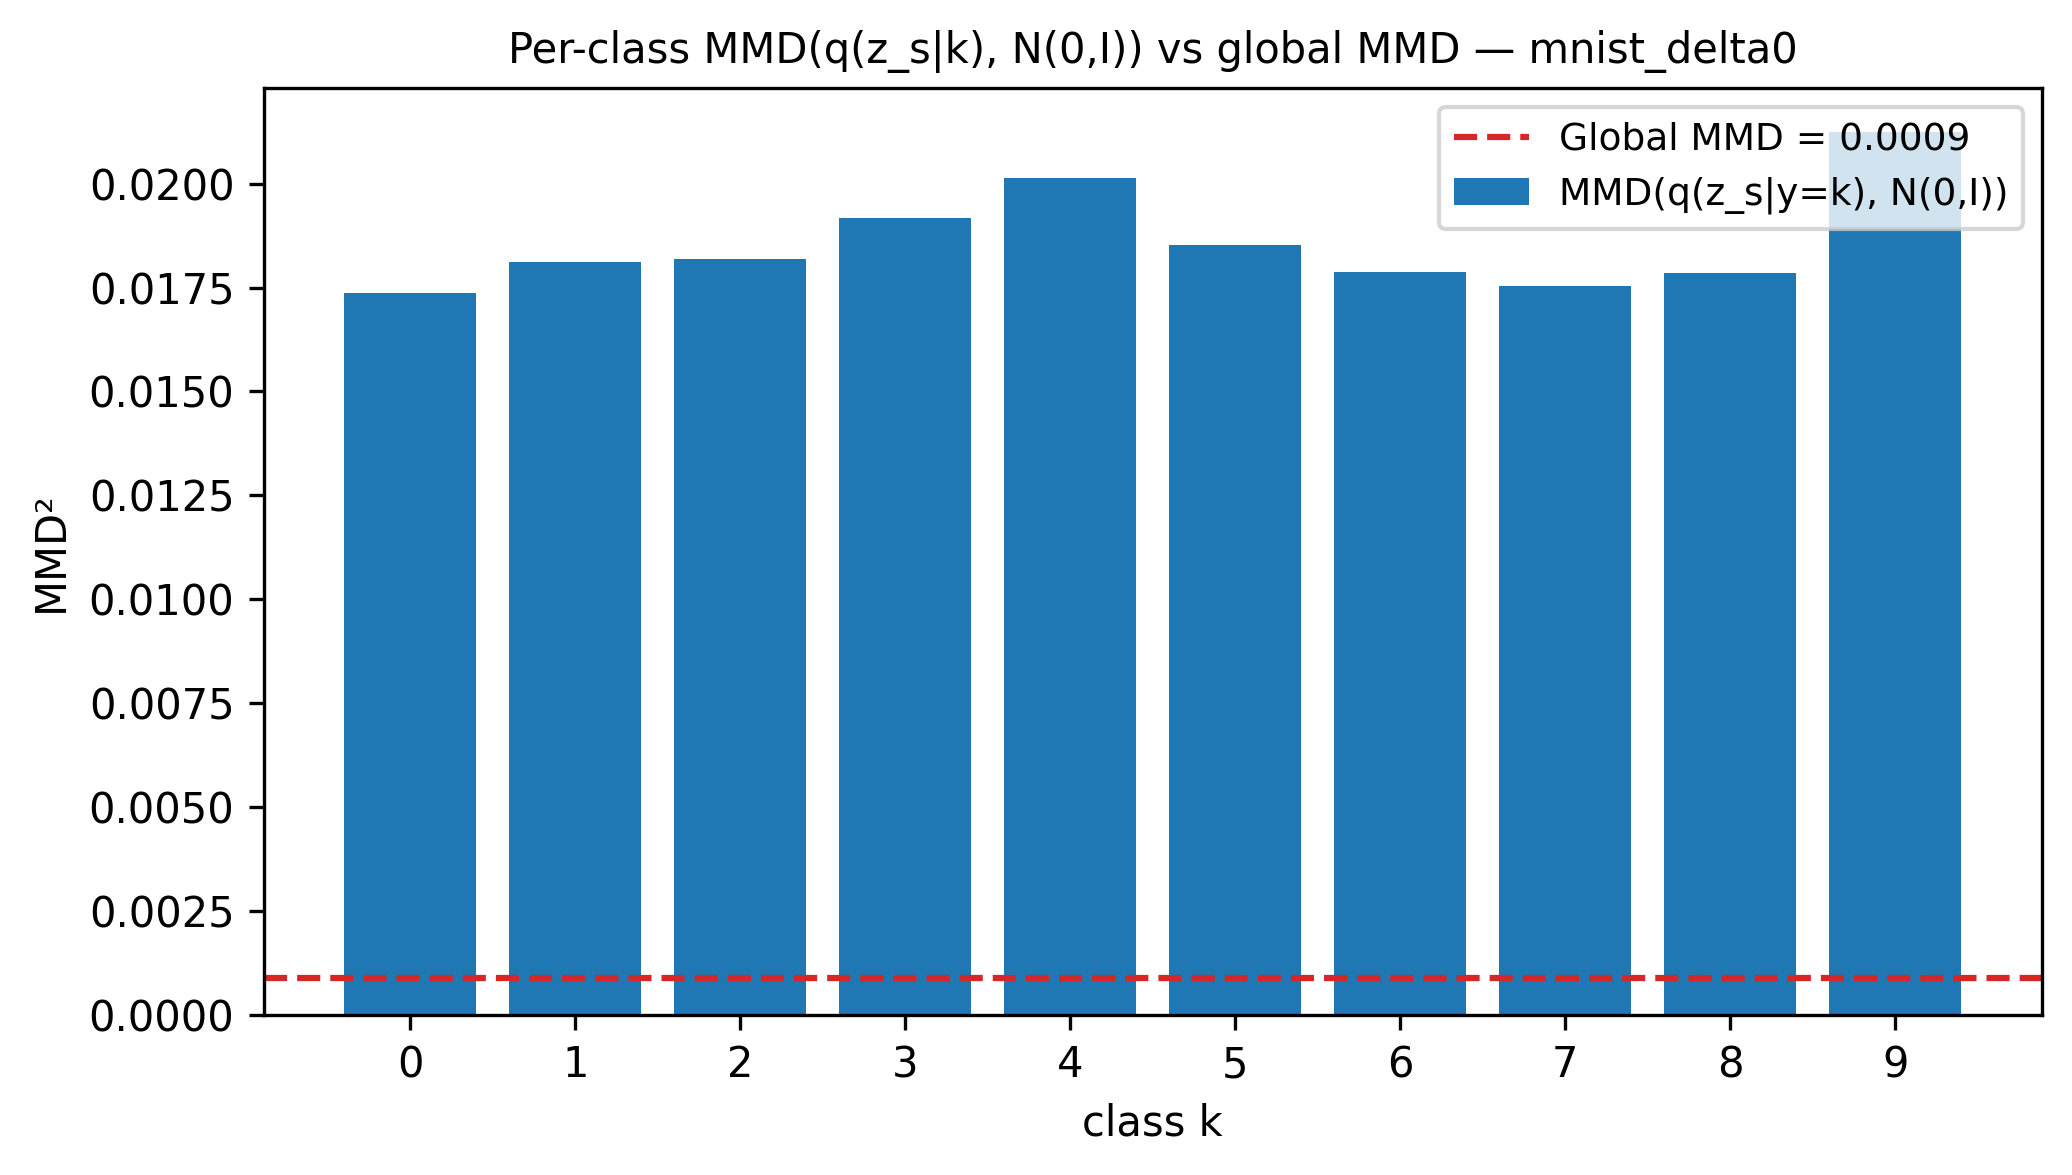
\includegraphics[width=\linewidth,trim=0 0 0 85,clip]{conditional_mmd_per_class_bar_mnist.png}\\[-0.5em]
\small (a) MNIST
\end{minipage}\hfill
\begin{minipage}{0.49\textwidth}
\centering
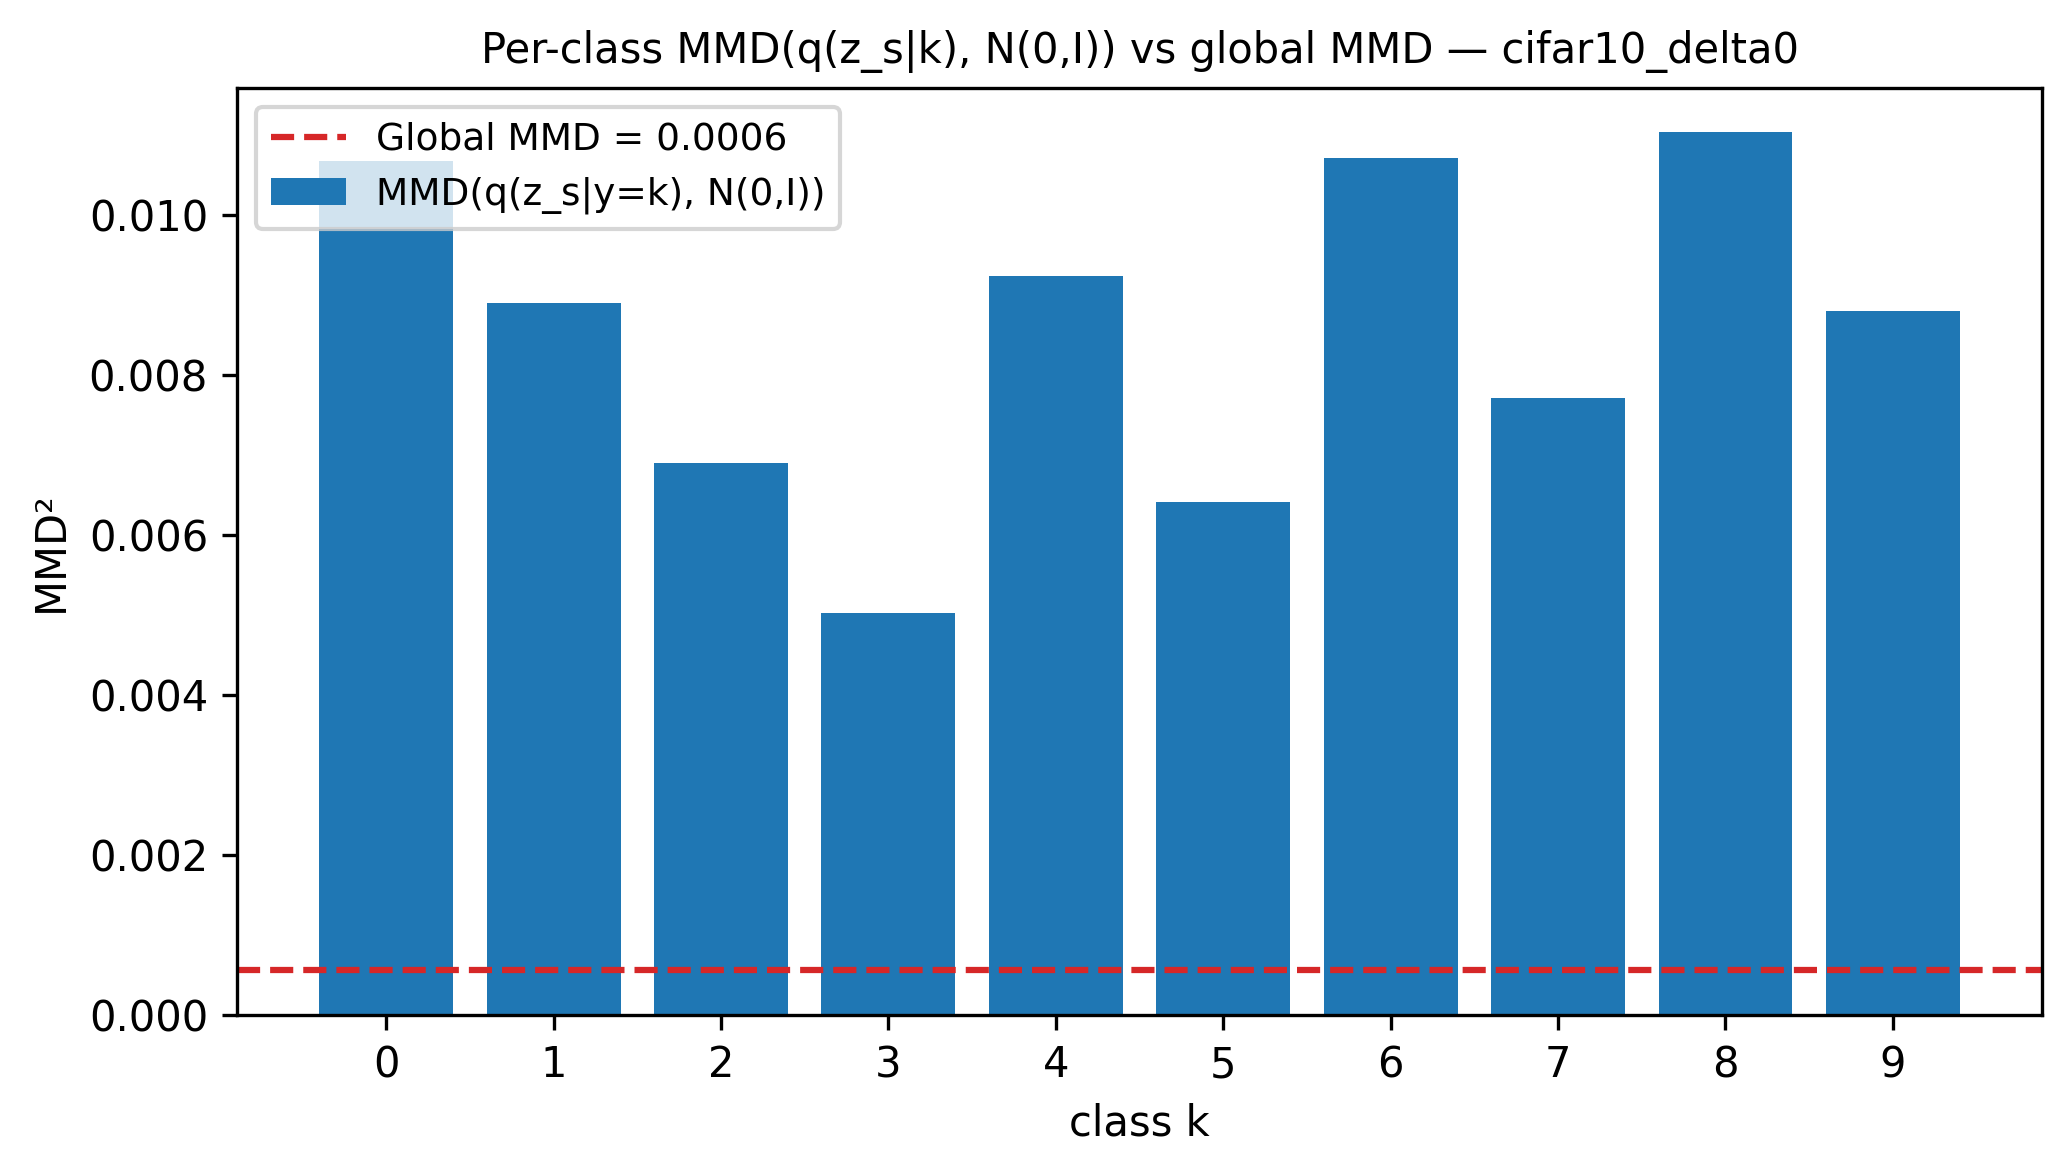
\includegraphics[width=\linewidth,trim=0 0 0 85,clip]{conditional_mmd_per_class_bar_cifar10.png}\\[-0.5em]
\small (b) CIFAR-10
\end{minipage}
\caption{Per-class $\MMD^2(q(\zs\mid y=k),\mathcal N(0,I))$ at
$\delta=0$ on stochastic posterior samples.  The dashed line is the global
$\MMD^2(q(\zs),\mathcal N(0,I))$ optimized by the marginal regularizer.
All ten conditional values exceed it on each dataset.}
\label{fig:conditional-mmd-bars}
\end{figure}

The per-class objective acts in the predicted direction: it reduces mean
conditional MMD by $87.6\%$ on MNIST and $86.5\%$ on CIFAR-10, and reduces
$\Dinter$ by $76.7\%$ and $64.9\%$, respectively.  It does not make either
conditional statistic vanish; global MMD remains below $10^{-3}$.  We do not
reuse the historical remedy probe accuracy here because those checkpoints
have not yet been regenerated with the held-out Stage-0 probe protocol.

The decomposition also predicts a distinct within-class failure.  We sample
$(\zc,\zs)$ ten times per checkpoint and apply classwise conditional HSIC
with within-class permutations.  Every draw rejects
$\zc\perp\zs\mid y$ on MNIST, Fashion-MNIST, and all three CIFAR-10 baseline
seeds ($p=1/201$).  Rejection also persists for the seed-0 $\delta=1$
checkpoints on MNIST and CIFAR-10.  This is a stochastic-view kernel test,
not an estimate of $I(\zc;\zs\mid y)$, but it directly demonstrates that
targeting term 2 does not complete the term-4 audit.
\FloatBarrier

\subsection{Conditional regularization has a non-monotone trade-off}

Table~\ref{tab:delta-sweep} shows four points from the six-value $\delta$
sweep.  Conditional separation decreases steadily, but clustering and FID
are not monotone.  On MNIST, the $\delta=1$ checkpoint has an isolated ACC
drop that disappears at $\delta=3$; on CIFAR-10, ACC drops at
$\delta=0.3$ and only partially recovers.  Because every sweep point is a
single training seed, these irregularities may be optimization noise and are
not evidence of a causal optimum.

\begin{table}[ht]
\caption{Selected points from the single-seed per-class-MMD sweep.  No
uncertainty or significance claim is made across settings.}
\label{tab:delta-sweep}
\centering
\small
\begin{tabular}{crrrrrr}
\toprule
& \multicolumn{3}{c}{MNIST} & \multicolumn{3}{c}{CIFAR-10} \\
$\delta$ & ACC & $\Dinter$ & FID & ACC & $\Dinter$ & FID \\
\midrule
0   & .992 & 6.21 & 74.0 & .813 & 3.74 & 80.5 \\
.1  & .990 & 2.12 & 52.6 & .810 & 2.03 & 77.5 \\
1   & .859 & 1.22 & 43.4 & .800 & 1.05 & 74.4 \\
3   & .993 & 1.18 & 41.5 & .799 & .95  & 76.1 \\
\bottomrule
\end{tabular}
\end{table}

Figure~\ref{fig:delta-fid} makes the non-monotonicity visible across all six
archived settings.  The sweep supports a limited conclusion: conditional regularization
consistently compresses class separation in style space, but reduced leakage
does not guarantee monotonic improvement in semantic clustering or image
quality.  It also illustrates why the four terms of
Theorem~\ref{thm:decomp} should be monitored separately.

\begin{figure}[t]
\centering
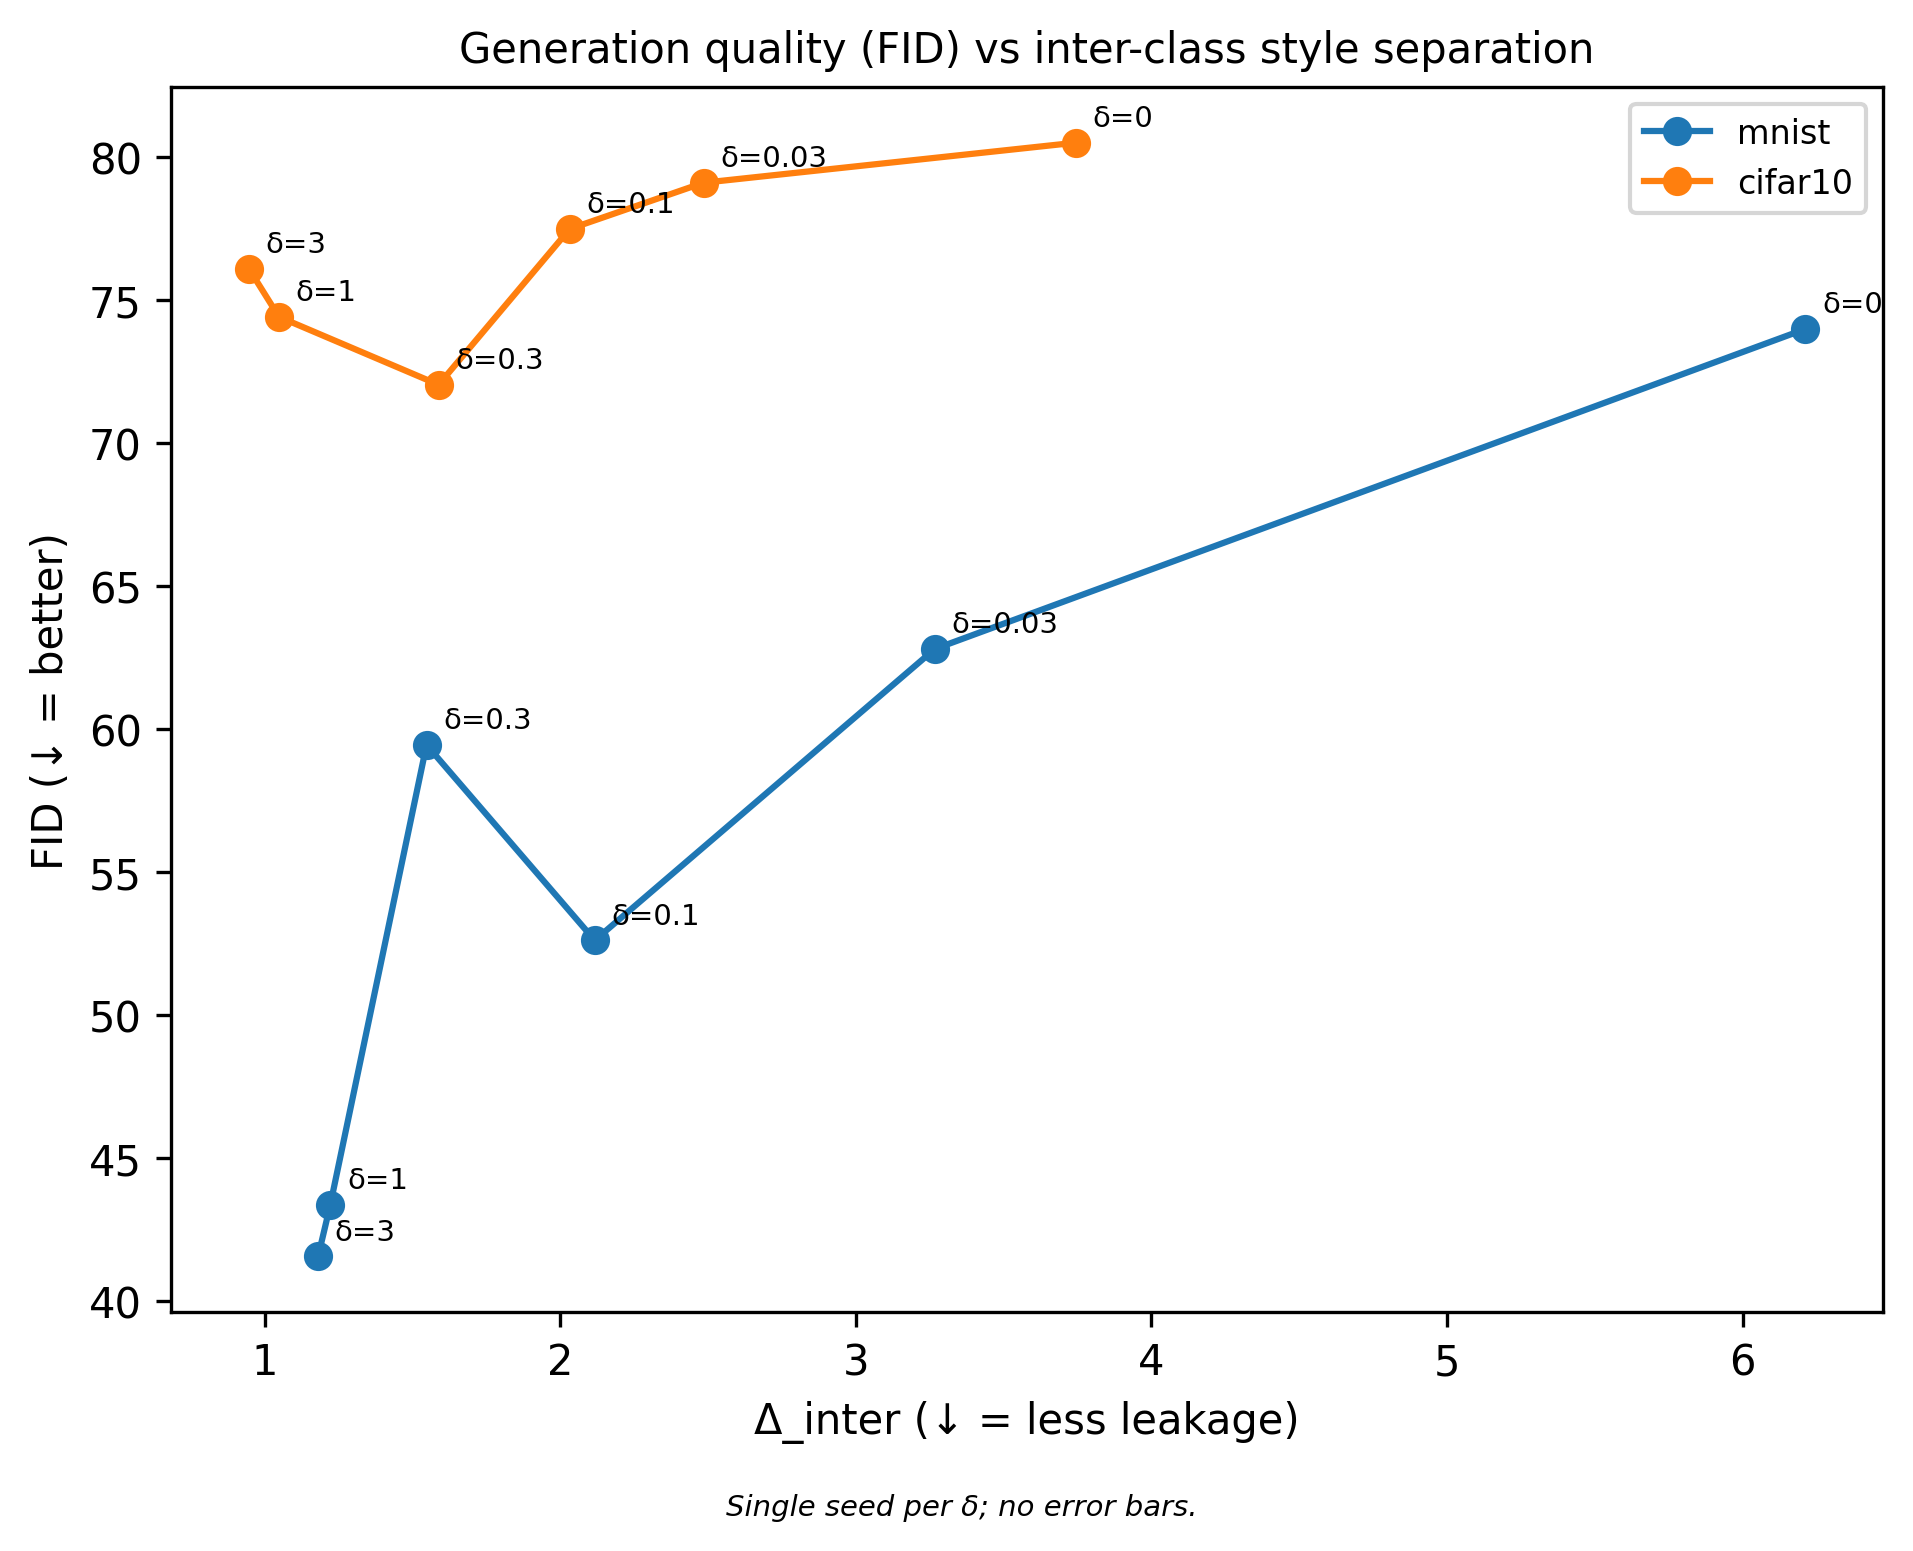
\includegraphics[width=0.55\textwidth,trim=0 0 0 65,clip]{delta_sweep_pareto_fid_deltainter.png}
\caption{Naive-prior FID against $\Dinter$ across all six single-seed
$\delta$ settings.  Connecting lines are visual aids, not claims of a smooth
response.  Conditional separation decreases steadily, whereas FID improves
overall but non-monotonically.}
\label{fig:delta-fid}
\end{figure}
\FloatBarrier

\subsection{The mismatch affects class-conditional generation}

We next test decoded samples using classifiers trained only on real pixels:
a four-layer CNN with $99.34\%$ MNIST test accuracy and a WideResNet-28-10
with $96.16\%$ CIFAR-10 test accuracy~\citep{zagoruyko2016wide}.  For a
requested class $k$, the naive sampler draws $\zc\sim p(\zc\mid k)$ and
$\zs\sim\mathcal N(0,I)$.  A post-hoc alternative fits a diagonal Gaussian
to encoded training styles from class $k$ and samples with temperature
$\tau=0.25$.  It uses labels and is a diagnostic workaround, not evidence
that the representation is disentangled.

\begin{table}[ht]
\caption{External generated-class accuracy under global and post-hoc
class-conditional style sampling.  The post-hoc distribution is fitted on a
training-only style bank; each checkpoint uses 1,000 generated images per
requested class.  CIFAR-10 is mean $\pm$ sample standard deviation over three
model seeds.}
\label{tab:generation}
\centering
\small
\begin{tabular}{lrr}
\toprule
Dataset & Global $\mathcal N(0,I)$ & Class diagonal, $\tau=0.25$ \\
\midrule
MNIST & 0.1047 & 1.0000 \\
CIFAR-10 & $0.1283\pm0.0032$ & $0.4716\pm0.0686$ \\
\bottomrule
\end{tabular}
\end{table}

Table~\ref{tab:generation} shows that respecting the learned
class-conditional style distribution substantially improves class identity,
especially on MNIST.  The smaller CIFAR-10 gain is consistent with a diagonal
conditional missing multimodal intra-class structure and with generally weak
sample quality; it should not be read as a complete repair.  A deterministic
mean-swap intervention isolates decoder dependence.  For off-diagonal donor
pairs at $\delta=0$, the external classifier follows the style donor in
$99.28\%$ of MNIST and $63.92\%$ of CIFAR-10 decodes, versus the semantic
donor in $0.06\%$ and $4.72\%$, respectively.  Per-class MMD reduces style-
following to $23.37\%$ and $35.92\%$, while increasing semantic-following;
these remedy comparisons remain single-seed mechanism checks.

\begin{figure}[ht]
\centering
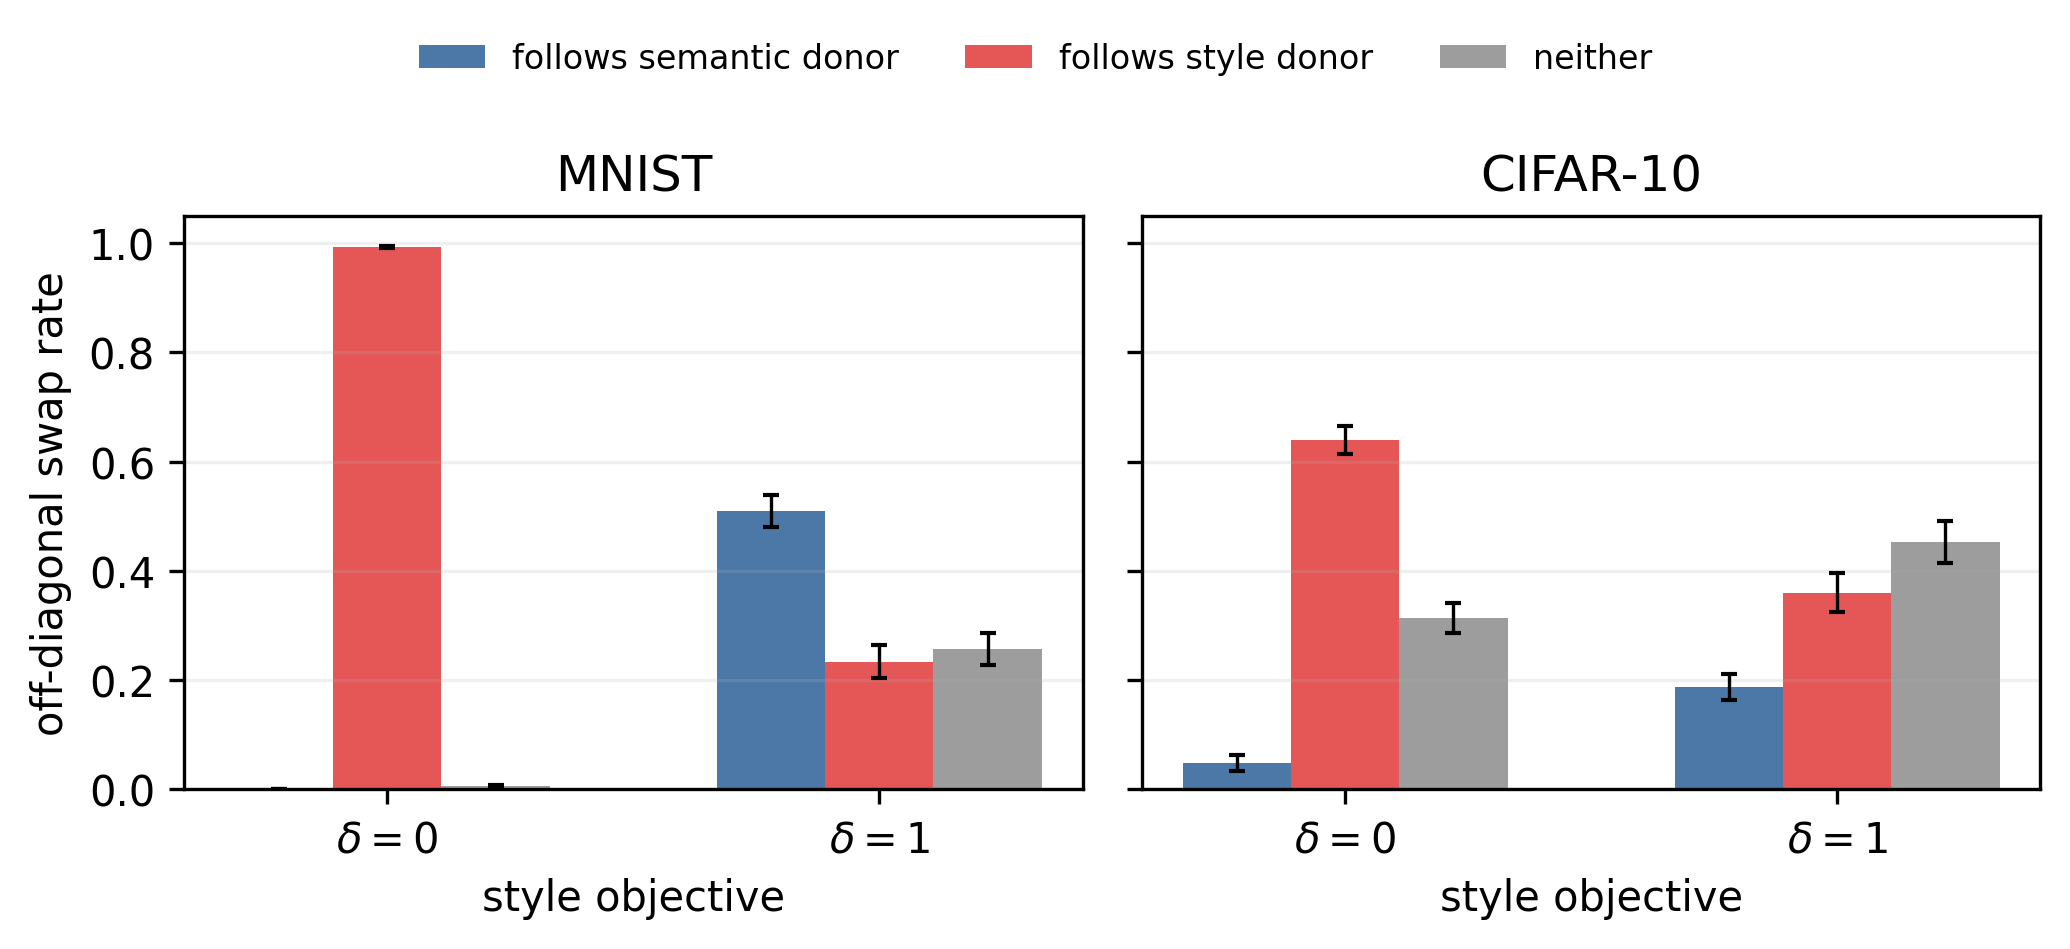
\includegraphics[width=0.78\textwidth]{external_swap_summary.png}
\caption{Independent-classifier outcomes for deterministic posterior-mean
swaps.  Bars average 90 ordered off-diagonal class pairs; intervals are 95\%
pair-bootstrap intervals.  At $\delta=0$, decoded identity predominantly
follows the style donor; per-class style MMD reduces, but does not eliminate,
this effect.}
\label{fig:external-swap}
\end{figure}

\fi

\paragraph{Evidence ladder and reporting rules.}

We use four complementary settings.  The synthetic experiment controls the
population marginal exactly.  The original image audit covers MNIST,
Fashion-MNIST, and CIFAR-10.  The native cross-model comparison uses paired
$-30^\circ/+30^\circ$ Rotated-MNIST domains and model seeds $\{0,1,2\}$.
Finally, Shapes3D supplies six known factors: shape is designated as content,
and floor hue, wall hue, object hue, scale, and orientation as style
\citep{deepmind2018shapes3d}.  All headline sampling-contract diagnostics use
stochastic posterior samples and held-out splits.

Unbiased $\MMD^2$ estimates may be negative under the null and are never
clipped.  A failure to reject exact equality is not called proof of equality.
HSIC uses plus-one permutation calibration; we report domain-level outcomes
rather than average $p$-values.  Shapes3D applies Holm correction separately
within the six content tests and six style tests.  Final epochs and audit
populations are fixed without selecting checkpoints on leakage metrics.

\subsection{Can exact marginal matching hide conditional information?}
\label{sec:synthetic}

The decomposition makes aggregate matching a clause rather than a certificate.
We first isolate that logical point by instantiating the smooth construction from
Proposition~\ref{prop:nocert} in 128 dimensions:
\begin{equation}
z\sim\mathcal N(0,I),\qquad
p(y=1\mid z)=\sigma(2\kappa z_1).
\end{equation}
The latent is sampled before the label, so $q_\kappa(z)=\mathcal N(0,I)$
exactly for every $\kappa$: term 1 is zero by the data-generating process, not
because a test fails to reject.  We use 50 replications of 2,048 samples, 499
MMD and HSIC permutations, and the same stratified 60/20/20 linear-probe
protocol as the checkpoint audit.

\begin{figure}[t]
\centering
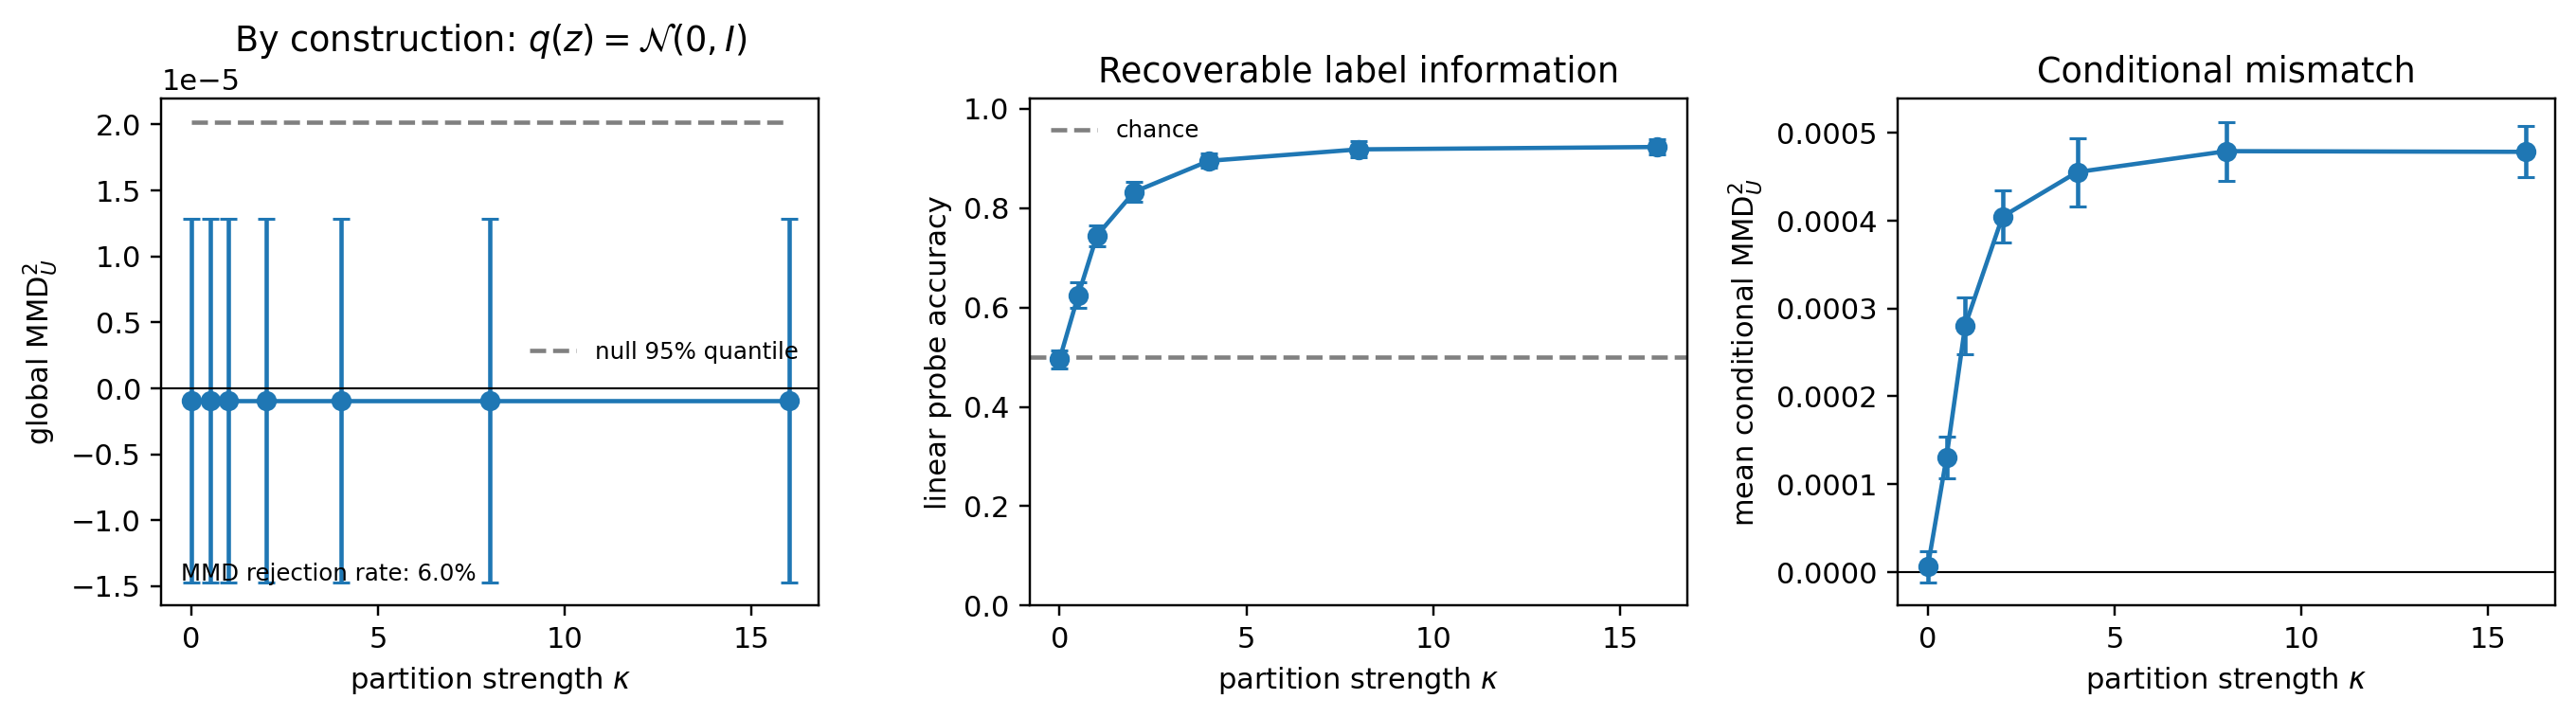
\includegraphics[width=0.98\textwidth]{exact_marginal_vs_leakage.png}
\caption{\textbf{Exact marginal matching does not certify label
independence.}  The same Gaussian sample is relabeled as partition strength
$\kappa$ changes.  Global MMD therefore remains invariant and rejects in
$3/50=6\%$ replications, compatible with its nominal $5\%$ level.  Meanwhile,
probe accuracy exceeds $90\%$ at $\kappa=8,16$ and conditional discrepancy
increases.  Points and bars are mean $\pm$ one standard deviation.}
\label{fig:exact-marginal}
\end{figure}

Probe accuracy rises from $49.58\!\pm\!1.86\%$ at $\kappa=0$ to
$92.30\!\pm\!1.51\%$ at $\kappa=16$.  HSIC rejects in $100\%$ of replications
for every $\kappa>0$, while its null rejection rate is $2\%$.  Mean
conditional MMD rises from $6.16\times10^{-6}$ to
$4.78\times10^{-4}$.  The preregistered eight-part composite gate did not
fully pass: the requirement of probe accuracy above $90\%$ at each of
$\kappa\in\{4,8,16\}$ missed at $\kappa=4$ ($89.51\%$, a 0.49-point gap).
All calibration and trend checks passed.  We preserve this failure and use
only the supported existential claim: exact marginal equality can coexist
with more than $90\%$ recoverable label information.

A sweep over $n=512$--$4096$ preserves $92.0$--$92.5\%$ probe accuracy and
$5$--$6\%$ global-MMD rejection (Appendix~\ref{tab:synthetic-n-v9}).
This stability is the expected pattern, not a failure of the sample-size
study.  At fixed $\kappa$, the population relation between $z_1$ and $y$---and
therefore the attainable classification accuracy---does not strengthen when
more observations are drawn.  Increasing $n$ should mainly stabilize its
finite-sample estimate.  More importantly, the marginal remains exactly
Gaussian for every $n$, so a valid level-.05 global test should continue to
reject only at roughly its nominal rate.  The sweep exhibits both properties:
the predictive effect is essentially unchanged and the marginal test does not
acquire spurious power against a null that is true by construction.
\FloatBarrier

\subsection{Does the audit distinguish qualitatively different failures?}
\label{sec:cross-model}

The construction establishes possibility, but learned models serve a different
role: they test whether the audit reports leakage indiscriminately or separates
practically different regimes.  We train native-family, common-backbone adaptations of F-CS-WAE,
DRIT~\citep{lee2018drit}, and DIVA~\citep{ilse2020diva} for 100 epochs on the
same two-domain Rotated-MNIST population.  The audited style variables are
F-CS-WAE $z_s$, DRIT's domain-specific attribute code, and DIVA's residual
$z_x$.  DRIT domains are audited separately because their attribute spaces
are domain-specific.

\begin{table}[t]
\caption{Native cross-model audit, mean $\pm$ sample standard deviation over
three model seeds.  Probe and retention entries are percentages.  ``Base''
checks reconstruction and content representation; ``all'' additionally
includes the preregistered $70\%$ prior-style retention gate.}
\label{tab:cross-model}
\centering
\scriptsize
\setlength{\tabcolsep}{3.2pt}
\resizebox{\textwidth}{!}{%
\begin{tabular}{lrrrrrrrr}
\toprule
Family & Global MMD & Cond. MMD & Logit $z_s$ & RBF $z_s$ & Content & Rec. L1 & Prior retain & Base / all \\
\midrule
F-CS-WAE & $.003326\!\pm\!.000140$ & $.032262\!\pm\!.001197$ & $91.92\!\pm\!2.43$ & $96.67\!\pm\!.95$ & $99.42\!\pm\!.14$ & $.01510\!\pm\!.00036$ & $12.37\!\pm\!1.19$ & $3/3$ / $0/3$ \\
DRIT & $.255261\!\pm\!.008545$ & $.272442\!\pm\!.001938$ & $34.42\!\pm\!12.62$ & $32.50\!\pm\!14.12$ & $88.25\!\pm\!1.52$ & $.04284\!\pm\!.00211$ & $9.87\!\pm\!.12$ & $3/3$ / $0/3$ \\
DIVA & $-.0000179\!\pm\!.0000274$ & $.000176\!\pm\!.000129$ & $10.67\!\pm\!1.04$ & $11.83\!\pm\!.63$ & $96.67\!\pm\!.76$ & $.03449\!\pm\!.00009$ & $89.45\!\pm\!.83$ & $3/3$ / $3/3$ \\
\bottomrule
\end{tabular}}
\end{table}

The audit separates three qualitatively different outcomes.  F-CS-WAE has a
roughly tenfold conditional/global discrepancy and high, seed-stable label
recovery.  DRIT's global discrepancy is already large, so its label-bearing
attribute code is a wholesale prior-sampler failure rather than a
matched-marginal paradox.  DIVA has near-null global discrepancy, chance-level
probes, and competent prior-style retention.  HSIC rejects in all six
seed-domain tests for F-CS-WAE and DRIT ($p=1/201$).  Two of six raw DIVA tests
fall below .05, but none survives Holm correction within the DIVA family and
the probe pattern does not repeat.  We therefore say that the audit finds no
stable, practically recoverable DIVA residual leakage at this power---not that
independence has been proven.

The frozen all-check gate is intentionally shown even though its retention
component is also an outcome of the sampling contract.  Post hoc, all three
families pass the separable reconstruction/content checks, while only DIVA
passes the full preregistered gate.  DRIT and DIVA are faithful
native-objective common-backbone adaptations, not exact reproductions of the
authors' benchmark architectures; this experiment supports audit
discrimination, not a ranking of the original methods.

\subsection{Is leakage only a consequence of posterior collapse?}
\label{sec:entropy}

F-CS-WAE's raw variance head often reaches its numerical floor.  To test
whether that alone creates leakage, we retrain MNIST seed 0 and CIFAR-10 seeds
$\{0,1,2\}$ with
\begin{equation}
\sigma_{\mathrm{eff}}^2(x)=
\exp(\operatorname{clamp}(\log\sigma_s^2(x),-10,10))+
\sigma_{\mathrm{floor}}^2,
\end{equation}
using the same sampler during training and audit.  Table~\ref{tab:entropy}
reports the complete fixed CIFAR-10 suite and representative MNIST points from
its five-level sweep.

\begin{table}[t]
\caption{Entropy intervention.  MNIST is seed 0; CIFAR-10 entries are rounded
three-seed means.  Probe/Gen-ACC are percentages; every CIFAR seed rejects
HSIC at $p=1/201$.}
\label{tab:entropy}
\centering
\scriptsize
\setlength{\tabcolsep}{3.5pt}
\resizebox{\textwidth}{!}{%
\begin{tabular}{llrrrrrrr}
\toprule
Data & $\sigma_{\rm floor}$ & $H$ & Probe & Global MMD & Cond. MMD & HSIC $p$ & Gen-ACC & Rec. \\
\midrule
MNIST & 0 & -3.581 & 99.76 & .000579 & .016024 & .00498 & 10.15 & .01259 \\
MNIST & .15 & -.477 & 98.78 & .000654 & .012044 & .00498 & 37.35 & .01520 \\
MNIST & .35 & .381 & 95.61 & .000518 & .007516 & .00498 & 93.50 & .01658 \\
\midrule
CIFAR-10 & 0 & -3.581 & 68.0 & .00030 & .0058 & .00498 & 13.0 & .052 \\
CIFAR-10 & .15 & -.477 & 29.0 & .00070 & .0037 & .00498 & 27.0 & .059 \\
CIFAR-10 & .35 & .369 & 10.5 & .00067 & .0013 & .00498 & 52.0 & .065 \\
\bottomrule
\end{tabular}}
\end{table}

On MNIST, increasing entropy by 3.96 nats/dimension still leaves $95.61\%$
label accuracy, while reconstruction loss remains only $1.32\times$ baseline.
On CIFAR-10, $\sigma_{\rm floor}=.15$ is a non-degenerate operating point:
the mean probe remains $19.0$ points above chance, conditional MMD is
$5.3\times$ global MMD, reconstruction increases by about $13.5\%$, and
Gen-ACC improves.  At $.35$, however, the mean linear probe is $10.5\%$,
effectively chance, even though every seed still rejects HSIC and conditional
MMD remains positive.  We therefore do not call this strong recoverable label
leakage.  The replicated boundary shows that added stochasticity attenuates
the failure without making near-determinism a necessary condition for it.
MNIST remains a single-seed intervention; the raw variance head remains
floor-seeking.

The high-noise CIFAR-10 result illustrates why test outcomes and effect sizes
must be reported together.  HSIC asks whether there is evidence of \emph{any}
dependence detectable by its kernel, whereas the logistic probe asks whether
label information is usefully recoverable through a particular linear
decision rule.  Consequently, $p=.00498$ at $\sigma_{\rm floor}=.35$ does not
contradict a $10.5\%$ probe: the representation can remain statistically
non-independent while carrying little linearly exploitable label signal.
The simultaneous fall in conditional MMD from $.0058$ to $.0013$ supports
attenuation, rather than an estimator-only explanation.  Gen-ACC rises as
this mismatch falls, but because every level is separately trained, we treat
that alignment as mechanism evidence rather than a causal estimate of the
effect of conditional MMD alone.

\subsection{Does the latent mismatch affect the decoder?}

A recoverable label in style matters operationally only if the decoder uses
it.  We therefore pair the original fixed audit on MNIST, Fashion-MNIST, and
CIFAR-10 with prior-sampling and donor-swap interventions.  Exact global
equality is rejected for every learned checkpoint, so ``small'' below is only
relative to conditional discrepancy; these models are not used to establish
the exact-marginal counterexample.

\begin{table}[t]
\caption{Original F-CS-WAE audit.  MMD/probe entries are rounded three-seed
aggregates; generation retains its original scope (MNIST seed 0, CIFAR three
seeds).  Every seed rejects HSIC at $p=1/201$.}
\label{tab:image-audit}
\centering
\small
\begin{tabular}{lrrrr}
\toprule
Dataset & Global MMD & Logit $z_s$ & Global Gen-ACC & Class-style Gen-ACC \\
\midrule
MNIST & .00058 & 99.6 & .1047 & 1.0000 \\
Fashion-MNIST & .00034 & 88.0 & --- & --- \\
CIFAR-10 & $.000298\!\pm\!.000052$ & $68.62\!\pm\!6.19$ & $.1283\!\pm\!.0032$ & $.4716\!\pm\!.0686$ \\
\bottomrule
\end{tabular}
\end{table}

Across the new three-seed aggregates, conditional MMD is $.0160$ on MNIST and
$.010$ on Fashion-MNIST; all seedwise HSIC tests attain $p=1/201$.  The
post-hoc class-style sampler is fitted on encoded training styles and is
a mechanism check, not a factorization repair.  Its gain shows that the
decoder is sensitive to the conditional mismatch.  Deterministic off-diagonal
mean swaps agree: decoded identity follows the style donor in $99.28\%$ of
MNIST and $63.92\%$ of CIFAR-10 cases, versus the semantic donor in $.06\%$
and $4.72\%$.

Archived seed-0 checkpoints provide a directional conditional intervention.
Adding the per-class style objective in Eq.~\ref{eq:perclass} reduces
style-donor following to $23.37\%$ on MNIST and $35.92\%$ on CIFAR-10 while
increasing semantic-donor following.  Yet conditional HSIC still rejects on
all ten stochastic posterior draws at $\delta=1$.  This does not prove that
fixing term 2 can never fix sampling; rather, the joint pattern is consistent
with Theorem~\ref{thm:decomp}: suppressing class-dependent style structure can
improve decoder behavior while leaving detectable term-4 coupling.  Because
the intervention is one seed, we treat it as mechanism evidence, not a remedy
benchmark.  Full probes, conditional MMD, and swap matrices are retained in
Appendix~\ref{app:full-results}--\ref{app:decoder}.

\FloatBarrier

\subsection{Does the pattern extend to explicit generative factors?}
\label{sec:shapes3d}

Shapes3D contains all combinations of six independent factors.  We train
F-CS-WAE, an observed-shape conditional VAE~\citep{sohn2015learning}, and a
learned supervised content--style VAE with class-conditional content priors
\citep{ilse2020diva}.  All use a native $64\times64$ decoder and the same
120k/20k/20k shape-stratified IID split at fixed epoch 100.  F-CS-WAE and the
learned VAE use seeds $\{0,1,2\}$; the oracle observed-shape cVAE remains the
predefined seed-0 control.  An
independent multi-head image evaluator passes every preregistered factor
threshold, and all three generators pass the reconstruction/content
competence gate.

\begin{table}[ht]
\caption{Shapes3D audit.  Except for seed-0 global MMD, F-CS-WAE/learned-VAE
entries are rounded three-seed means; the observed-shape cVAE is seed 0.
$z_c\!\to$style averages five nuisance-factor probes.}
\label{tab:shapes3d}
\centering
\scriptsize
\setlength{\tabcolsep}{3.2pt}
\resizebox{\textwidth}{!}{%
\begin{tabular}{lrrrrrrr}
\toprule
Model & Global MMD ($p$) & Cond. shape MMD & $z_s\!\to$shape & $z_c\!\to$style & Prior shape retain & Swap shape retain & Rec. L1 \\
\midrule
F-CS-WAE & $.000766$ (.002) & .0085 & 99.0 & 87.0 & 89.0 & 88.0 & .0023 \\
Observed-shape cVAE & $.000026$ (.092) & .000076 & 25.98 & 10.17 & 99.88 & 100.00 & .00260 \\
Learned C/S VAE & $-.0000005$ (.501) & .00004 & 25.5 & 9.5 & 99.7 & 99.8 & .0029 \\
\bottomrule
\end{tabular}}
\end{table}

Across three seeds, F-CS-WAE style predicts shape at $99.0\%$ and its content
predicts nuisance factors at $87.0\%$.  At seed 0, HSIC rejects all six factor
tests in each view after Holm correction.  By contrast, both controls
place style-to-shape probes near chance and retain no Holm-significant shape
dependence in style; their content codes reject only for shape, while their
style codes reject for the five intended nuisance factors.  Across three
seeds, prior-style and posterior-swap decodes preserve shape at $99.7\%$ and
$99.8\%$ for the learned control but only $89.0\%$ and $88.0\%$ for F-CS-WAE.
Thus the class-label finding is not
merely an arbitrary semantic proxy in this controlled setting: the designated
shape factor cross-loads into style, while nuisance factors cross-load into
content.

\begin{figure}[ht]
\centering
\begin{minipage}{0.49\textwidth}
\centering
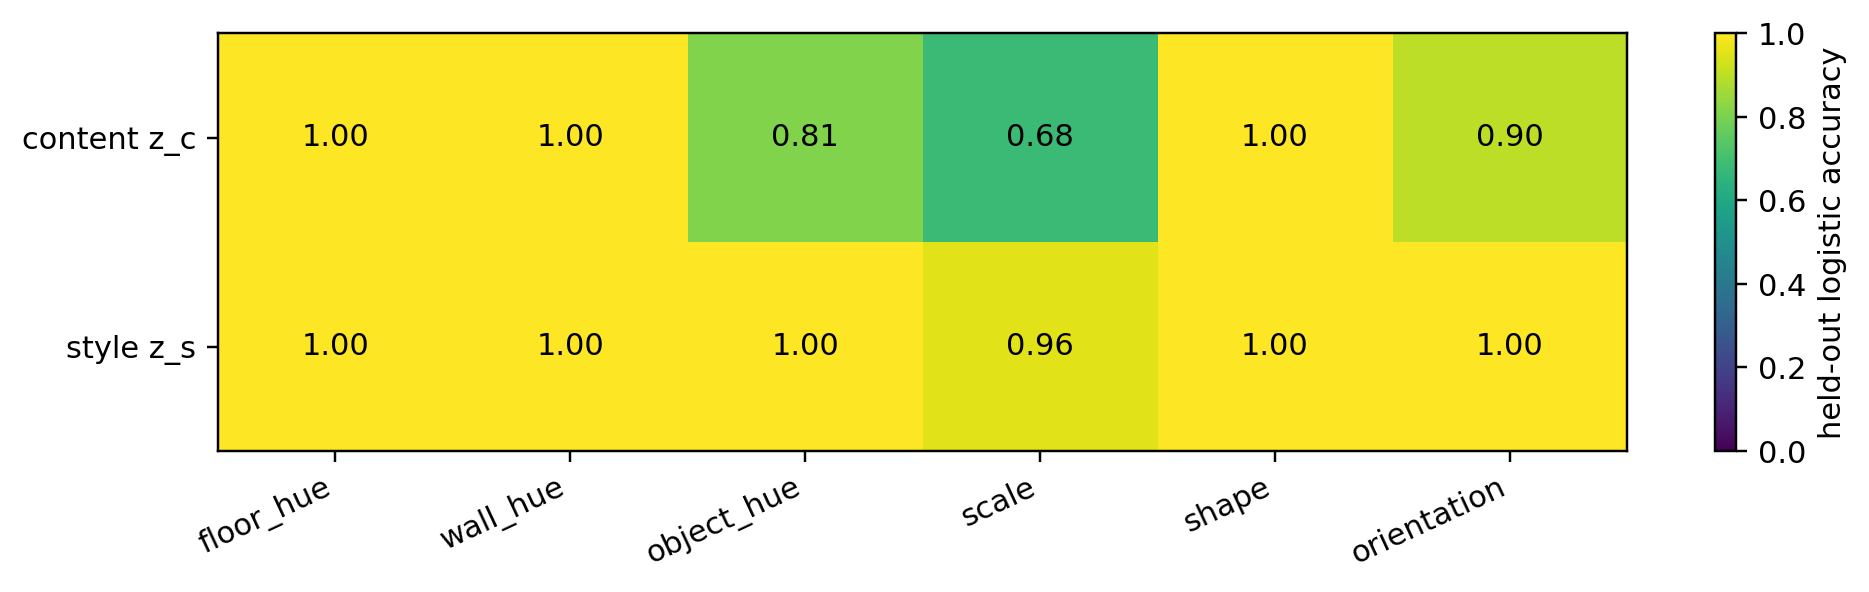
\includegraphics[width=\linewidth]{shapes3d_fcswae_factor_loading.png}\\[-0.5em]
\small (a) F-CS-WAE
\end{minipage}\hfill
\begin{minipage}{0.49\textwidth}
\centering
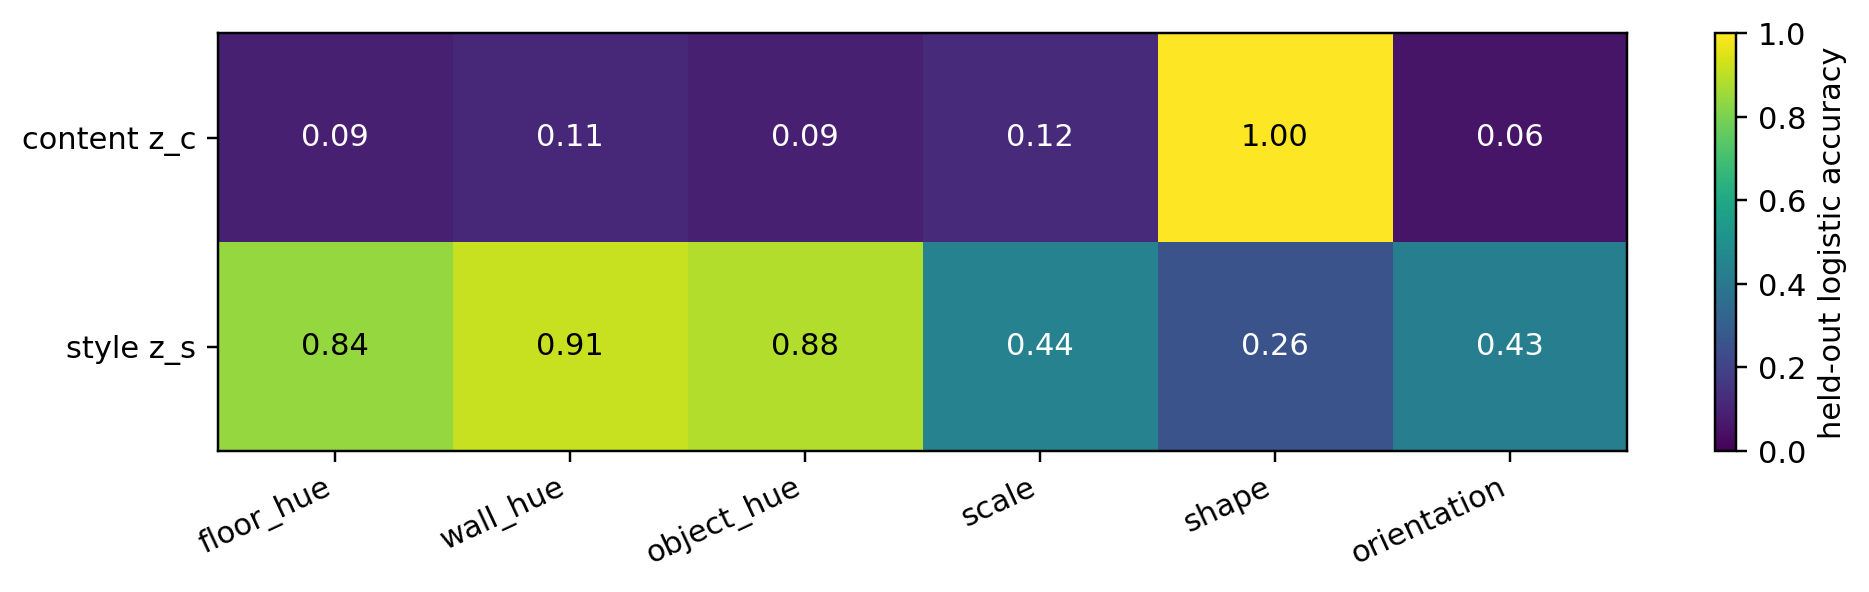
\includegraphics[width=\linewidth]{shapes3d_content_style_vae_factor_loading.png}\\[-0.5em]
\small (b) learned content--style VAE
\end{minipage}
\caption{Held-out factor loading on Shapes3D stochastic latents.  F-CS-WAE
stores nearly every factor in both codes; the learned VAE places shape in
content and nuisance factors in style.  Accuracy is descriptive; the text
reports Holm-corrected HSIC.}
\label{fig:shapes3d-loading}
\end{figure}

The F-CS-WAE/learned-control contrast repeats over three predefined seeds on
an IID factor split.  It establishes seed-level replication under that split,
not compositional generalization to unseen factor combinations; the
observed-shape oracle remains a single-seed auxiliary control.

The controls are essential to this interpretation.  A probe near $25\%$ on
the four-way shape task shows that the audit does not automatically extract
shape from every style code, while $99.7$--$99.8\%$ retention shows that the
same evaluator can recognize preserved shape after prior sampling and swaps.
F-CS-WAE instead combines a $99.0\%$ style-to-shape probe with only
$89.0\%$ prior and $88.0\%$ swap retention.  Thus the latent diagnostic and
the decoded intervention point in the same direction: shape is cross-loaded
into style, and breaking the encoded pairing changes shape more often.  The
learned VAE is not proof of perfect disentanglement, but it is a concrete
negative control showing that this protocol can recover the intended split.
\FloatBarrier

\section{Discussion and Limitations}
\label{sec:discussion}

\iffalse % v8 discussion retained in source provenance only

\subsection{What the evidence chain establishes}

The decomposition separates a logically necessary condition from an
empirical failure.  Proposition~\ref{prop:nocert} shows that marginal matching
cannot certify independence in any model.  Table~\ref{tab:stage0} shows the
gap in actual stochastic posterior samples.  Table~\ref{tab:generation}
and Figure~\ref{fig:external-swap} then connect the discrepancy to decoded
class identity through sampling and intervention.

Each step rules out a different, weaker explanation.  The global-versus-
conditional MMD comparison rules out interpreting a small mixture-level
statistic as evidence that every class component matches the prior.  Held-out
linear and nonlinear probes, together with permutation-calibrated HSIC, show
that the discrepancy is label-structured rather than merely an arbitrary
distributional deviation.  Repeating the audit on stochastic samples rules
out a mean-only probing artifact for these checkpoints.  Finally, the
external generated-class evaluator connects the latent discrepancy to the
sampler's observable output rather than relying on re-encoded samples.  No
single diagnostic makes all four points.

The conditional-MMD intervention is supportive but deliberately secondary.
It moves conditional MMD and class-mean separation in the direction predicted
by term 2, while leaving global MMD almost unchanged.  However, its sweep is
single-seed, its quality metrics are non-monotone, and its post-hoc sampling
counterpart uses labels.  We therefore treat it as a mechanism check, not as
a new disentanglement method or a tuned remedy benchmark.

\subsection{Implications for evaluating factorized samplers}

Theorem~\ref{thm:decomp} suggests a minimal reporting standard.  First, state
the joint distribution that the decoder receives during encoding and the
distribution used at generation; otherwise the claimed factorization has no
testable contract.  Second, identify whether each diagnostic uses posterior
means, posterior samples, or prior samples.  Third, report both aggregate fit
and a conditional dependence statistic on held-out data.  Fourth, examine
within-class dependence between the proposed factors instead of stopping once
style is label-invariant.  Fifth, evaluate the final decoded samples with an
external endpoint that was not trained jointly with the generator.  The goal
is not to estimate all four KL terms, but to align each proxy with the
equality it tests.

\subsection{Limitations and threats to validity}

Several limitations bound the present evidence.  First, class labels are a
proxy for semantic content, not a complete definition of content.  Datasets
with known pose, lighting, shape, or color factors are needed to test both
directions of disentanglement.  Second, MNIST and Fashion-MNIST currently have
one model seed, while CIFAR-10 has three.  Third, the almost deterministic
style posterior may amplify leakage and motivates a controlled posterior-
entropy ablation.  Fourth, global and conditional MMD are finite-sample
kernel statistics, not KL or mutual-information estimates.  Fifth, generated
class accuracy depends on an external classifier and does not measure sample
quality or diversity.  Finally, Eq.~\ref{eq:perclass} is supervised and only
targets term 2; even perfect conditional matching would leave terms 3 and 4
unresolved.

There are also finite-sample and model-selection threats.  MMD and HSIC depend
on kernel bandwidths and have limited power in high dimension; our multiscale
kernels and permutation calibration reduce sensitivity to a single bandwidth
but do not remove it.  The probe split prevents test-set fitting, yet five
checkpoints are insufficient to characterize training variability outside
CIFAR-10.  Generated-class accuracy can be biased by the external classifier's
decision boundary, so it should be paired with precision--recall or an
equivalent diversity-sensitive measure in a definitive study.  The present
results are strongest as a falsification of the independence claim for these
checkpoints, not as an estimate of how often the failure occurs across model
families.

Our current scope is therefore an audit of a concrete factorized model, not a
claim that all architectures fail at the same magnitude.  The practical
recommendation is correspondingly narrow: when independent style sampling
requires $\zs\perp y$, report a conditional dependence test on stochastic
samples in addition to aggregate prior fit, and verify whether the decoder
uses the detected information.

\fi

\subsection{What the contract and evidence establish}

The central result is the contract, not the observation that marginals and
conditionals differ.  Theorem~\ref{thm:decomp} characterizes exactly what is
changed when an encoded pair from $q(\zc,\zs\mid y)$ is replaced by an
independent draw from $p(\zc\mid y)p(\zs)$.  Proposition~\ref{prop:nocert} and
the synthetic experiment then serve the narrower purpose of showing that
perfect clause-1 satisfaction leaves clause 2 unconstrained.

The learned-model evidence evaluates whether this formal distinction is
operationally useful.  It supports three conclusions.  First, F-CS-WAE shows
conditional failure across original image checkpoints, three controlled
Rotated-MNIST seeds, a three-seed CIFAR-10 entropy intervention, and a
three-seed known-factor Shapes3D replication.  Second, the audit is
discriminative rather than universally positive: it separates that regime
from DRIT's aggregate-prior failure and DIVA's near-null boundary case, while
the Shapes3D VAE controls place the designated semantic factor in the intended
code.  Third, prior sampling and donor swaps connect latent findings to decoder
behavior instead of assuming every detectable mismatch must affect pixels.

None of these results says that every factorized model leaks, that a
non-rejection proves independence, or that probe accuracy equals mutual
information.  Likewise, a decoder can ignore a latent mismatch, so the
four-term KL decomposition is an upper-level contract, not a claim that every
nonzero latent statistic must visibly corrupt pixels.  This is why the audit
pairs prior and conditional statistics with independent pixel evaluators and
interventions.

\paragraph{A minimal sampling-contract audit.}
For a proposed sampler, report: (i) the encoded joint and generation-time
product; (ii) global prior fit on stochastic posterior samples; (iii) held-out
conditional probes and a calibrated dependence test; (iv) within-content
dependence; and (v) prior or swap outcomes scored by an independent evaluator.
Name posterior means, posterior samples, and prior samples explicitly.  On
known-factor data, audit both directions: content should not predict designated
style factors, nor style predict designated content.  The cross-model and
entropy results show why the full pattern is preferable to one scalar score:
aggregate failure, recoverable leakage, weak residual dependence, and a
near-null result call for different conclusions.

\subsection{Limitations and threats to validity}

The scope remains bounded.  The MNIST entropy sweep and the observed-shape
Shapes3D oracle use one training seed; the CIFAR-10 entropy sweep and the
F-CS-WAE/learned-VAE Shapes3D comparison use three.  Shapes3D uses an IID
shape-stratified split rather than unseen combinations.  DRIT and DIVA are
native-objective common-backbone
adaptations on one controlled two-domain dataset, not official benchmark
reproductions.  The Shapes3D pixel evaluator may share inductive biases with
the audited encoders despite being trained independently.  Decoder
interventions on MNIST remain seed 0.  The externally completed follow-ups are available here as rounded aggregate
exports, so we do not infer missing standard deviations from headline means.

MMD and HSIC remain kernel- and power-dependent finite-sample statistics, not
KL or mutual-information estimates.  Holm
correction controls the declared Shapes3D and DIVA test families but does not
turn failure to reject into equivalence.  Finally, labels and Shapes3D factors are controlled
definitions of content; conclusions need not transfer to dependent factors
in natural data.

\section{Conclusion}

Independent factorized generation makes a joint claim: the encoded
$q(\zc,\zs\mid y)$ must be replaceable by $p(\zc\mid y)p(\zs)$.  The
four-term decomposition exposes its clauses; term-aligned diagnostics
distinguish aggregate failure, conditional leakage, coupling, and near-null
results.  The exact construction establishes clause-wise insufficiency, while
trained-model and decoder evidence establish its operational value.

\clearpage
\section*{Reproducibility Statement}

Section~\ref{sec:protocol} specifies the core latent views, preprocessing,
probe selection, and permutation calibration.  Sections~\ref{sec:synthetic}--
\ref{sec:shapes3d} state the setting-specific populations, seeds, and fixed
reporting rules.  Appendix~\ref{app:proofs} contains complete proofs;
Appendices~\ref{app:protocol}--\ref{app:decoder} retain the original
checkpoint audit; and Appendices~\ref{app:synthetic-v9}--
\ref{app:shapes3d-v9} provide the expanded protocols, per-level/per-seed
results, multiplicity rules, competence gates, and artifact boundaries.
Unrounded seed-0 and cross-model values are tied to JSON manifests; newly
completed sample-size and three-seed follow-ups are identified as rounded
aggregates.  An anonymous supplementary archive will include the manifests,
follow-up aggregate exports, frozen criteria, and figure sources.

\section*{Ethics Statement}

This work uses standard public computer-vision benchmarks and existing model
checkpoints, collects no new data, and involves no human subjects or sensitive
personal information.  Its purpose is to identify and measure a failure mode
in factorized generative models.  Generated examples are low-resolution
benchmark images; nevertheless, the broader recommendation---auditing whether
a decoder uses unintended latent information---may also help identify
representation leakage in higher-stakes applications.

\section*{AI Use Statement}

Generative AI tools were used to provide feedback on evaluation methodology
and experimental design, assist with interpretation of diagnostic results,
audit consistency between implementation artifacts and reported procedures,
and help restructure and edit the manuscript.  They were not used to generate
datasets or experimental measurements.  The authors inspected the cited
literature, verified the mathematical arguments, executed and tested the
code, checked the experimental artifacts and every reported numerical value,
and reviewed all AI-assisted text.  The authors take responsibility for the
final content of this work.

\clearpage
\bibliographystyle{../iclr2027/iclr2027_conference}
\bibliography{references}

\appendix
\section{Proofs}
\label{app:proofs}

\subsection{Proof of Proposition~\ref{prop:nocert}}

The label is defined after drawing $\zs$ and therefore does not alter the
marginal law of $\zs$.  Hence $q(\zs)=\mathcal N(0,I)$ and any divergence
between these two identical measures is zero.  Because $y$ is a deterministic
function of $\zs$, $H(y\mid\zs)=0$.  The equal-probability partition gives
$H(y)=\log K$, and consequently
$I(\zs;y)=H(y)-H(y\mid\zs)=\log K$.

\subsection{A smooth, full-support construction}

Let $z\sim\mathcal N(0,1)$ and, conditional on $z$, draw a binary label with
\begin{equation}
P(y=1\mid z)=\sigma(az),\qquad P(y=0\mid z)=\sigma(-az),
\end{equation}
where $a>0$ and $\sigma(t)=(1+e^{-t})^{-1}$.  Since the standard normal
density $\phi$ is symmetric and $\sigma(t)+\sigma(-t)=1$,
\begin{align}
P(y=1)
&=\int_{\mathbb R}\phi(z)\sigma(az)\,dz\\
&=\frac12\int_{\mathbb R}\phi(z)
\bigl[\sigma(az)+\sigma(-az)\bigr]\,dz=\frac12.
\end{align}
The generative construction starts with the standard normal and changes only
the conditional label law, so the marginal of $z$ remains exactly standard
normal.  Bayes' rule gives
\begin{equation}
q(z\mid y=1)=2\phi(z)\sigma(az),\qquad
q(z\mid y=0)=2\phi(z)\sigma(-az).
\end{equation}
Both densities are smooth and strictly positive on $\mathbb R$.  When
$a\rightarrow\infty$, the conditional label approaches the indicator of the
sign of $z$ outside a set of Gaussian measure zero.  Thus
$H(y\mid z)\rightarrow0$ and $I(z;y)\rightarrow\log2$ while the marginal
remains unchanged.

\subsection{Proof of Theorem~\ref{thm:decomp}}

For a fixed $y$, insert the product of the encoder conditionals and apply the
KL chain rule:
\begin{align}
&\KL\!\left(q(\zc,\zs\mid y)\|p(\zc\mid y)p(\zs)\right)\\
={}&\KL\!\left(q(\zc,\zs\mid y)\|q(\zc\mid y)q(\zs\mid y)\right)\nonumber\\
&+\KL(q(\zc\mid y)\|p(\zc\mid y))
+\KL(q(\zs\mid y)\|p(\zs)).
\end{align}
The first term is $I_q(\zc;\zs\mid y)$ at that label.  Averaging over
$q(y)$ gives term 4 and term 3 of Eq.~\ref{eq:decomp}.  For the last term,
insert the aggregate posterior $q(\zs)$:
\begin{align}
\mathbb E_{q(y)}\KL(q(\zs\mid y)\|p(\zs))
={}&\mathbb E_{q(y)}\KL(q(\zs\mid y)\|q(\zs))\nonumber\\
&+\KL(q(\zs)\|p(\zs))\\
={}&I_q(\zs;y)+\KL(q(\zs)\|p(\zs)).
\end{align}
This establishes the equality for arbitrary $q(y)$.  Non-negativity follows
from non-negativity of KL divergence and mutual information.

\subsection{Proof of Corollary~\ref{cor:valid}}

An expectation of a non-negative KL is zero iff its integrand is zero for
$q(y)$-almost every $y$, which holds iff the two latent conditional measures
are equal.  The pushforward inequality follows by applying the data-processing
inequality to the deterministic Markov kernel induced by the decoder for each
$y$, then averaging over $q(y)$.

\section{Architecture and Training}
\label{app:model}

\subsection{Architecture}

The shared encoder is a ResNet-18 adapted to small images: its first
$7\times7$, stride-2 convolution is replaced by a $3\times3$, stride-1
convolution and max pooling is removed.  The trunk output is flattened and
mapped to 256 dimensions with SiLU.  Separate heads produce an unnormalized
semantic direction, a scalar semantic concentration, a style mean, and a
style log variance.  We use
\begin{align}
\muc&=\widetilde\muc/\|\widetilde\muc\|_2, &
\rho_c&=\sigma(r_c)(1-\varepsilon),\\
\zs&=\mus+\exp(\tfrac12\log\sigma_s^2)\odot\epsilon,
&\epsilon&\sim\mathcal N(0,I).
\end{align}
The semantic code is sampled by a Spherical Cauchy M\"obius
reparameterization.  The decoder concatenates $[\zc;\zs]$, projects it to a
$512\times4\times4$ tensor, and applies three residual bilinear-upsample
blocks with channel widths $256,128,64$.  Its sigmoid output is interpolated
to the native dataset resolution when necessary.  MNIST and Fashion-MNIST
therefore remain $28\times28$ and single-channel; CIFAR-10 remains
$32\times32\times3$.

For class $k$, the semantic prior is a Spherical Cauchy distribution centered
at an EMA direction $m_k$, with concentration $\rho_p=0.7$.  The center is
updated once per epoch from encoded class-mean directions with momentum
$0.95$.  The style prior is $\mathcal N(0,I)$.

\subsection{Objective}

The training objective is
\begin{align}
\mathcal L={}&\mathcal L_{\mathrm{rec}}
+\alpha(t)\mathcal L_{\mathrm{class}}
+\beta(t)\mathcal L_{\mathrm{agg}}
+\gamma(t)\mathcal L_{\mathrm{style}}\nonumber\\
&+\delta(t)\mathcal L_{\mathrm{style-cls}}
+\eta(t)\mathcal L_{\mathrm{cls}}.
\end{align}
$\mathcal L_{\mathrm{rec}}$ is L1 plus $0.1$ LPIPS
\citep{zhang2018unreasonable}.  $\mathcal L_{\mathrm{class}}$ matches each
semantic class conditional to its spherical prior, $\mathcal L_{\mathrm{agg}}$
matches aggregate semantic codes to the class-prior mixture,
$\mathcal L_{\mathrm{style}}$ matches sampled style codes to a standard
Gaussian, and $\mathcal L_{\mathrm{cls}}$ is cross entropy from $\muc$.
The baseline checkpoints audited in the main paper explicitly set
$\delta=0$; the repository default for new remedied runs is $\delta=1$, so
the run manifest or command-line override is required to distinguish them.

\begin{table}[ht]
\caption{Case-study training hyperparameters.}
\label{tab:hyperparameters}
\centering
\small
\begin{tabular}{ll}
\toprule
Parameter & Value \\
\midrule
Optimizer & Adam, learning rate $10^{-3}$ \\
Schedule & StepLR, step 100, factor $0.5$ \\
Batch size / epochs & 128 / 300 \\
Gradient clipping & global norm 1.0 \\
Semantic / style dimension & 64 / 128 \\
Semantic-prior concentration & 0.7 \\
EMA momentum & 0.95 \\
Final class / aggregate MMD weights & 2.0 / 5.0 \\
Final global style MMD weight & 1.0 \\
Final auxiliary-classifier weight & 0.3 \\
\bottomrule
\end{tabular}
\end{table}

Training has four phases: reconstruction only for epochs 0--49; global style
MMD and the auxiliary classifier ramp during epochs 50--99; semantic class
and aggregate MMD ramp to half strength during epochs 100--199; all terms
reach full strength during epochs 200--299.  For remedied runs, per-class
style MMD follows the global-style ramp.  No image augmentation is used.

\section{Canonical Audit Protocol}
\label{app:protocol}

\subsection{Data split and latent views}

For each checkpoint we select 2,048 examples from the standard test split
with evaluation seed 0.  Probe indices are generated by a deterministic
stratified 60/20/20 split, yielding 1,228 training, 410 validation, and 410
test examples.  Standardization parameters are estimated only on the 1,228
probe-training examples.  The split indices are stored by SHA-256 hash in
each result manifest.

The encoder is evaluated once to obtain $(\muc,\mus,\log\sigma_s^2)$ and a
seeded stochastic draw $\zs$.  We use:
\begin{itemize}
    \item $\mus$ for representation probes and deterministic mean swaps;
    \item $\zs$ for global MMD, conditional style statistics, and the
    sampling-contract probe; and
    \item both $(\muc,\mus)$ and repeated posterior draws $(\zc,\zs)$ for
    the conditional-dependence diagnostic.
\end{itemize}
Agreement between these views is reported as an empirical result rather than
assumed.

\subsection{Probe suite}

The suite contains multinomial logistic regression, a fixed two-layer MLP,
RBF-SVM, and $k$-NN.  Validation data are used for fixed early-stopping or
model-selection rules; every headline accuracy is evaluated once on the
untouched test partition.  We report accuracy and macro-F1.  The main paper
uses logistic regression as the simplest standardized headline and includes
RBF-SVM to detect nonlinear separation.

\subsection{MMD and HSIC}

Global MMD is the unbiased U-statistic with the averaged Euclidean RBF kernel
\begin{equation}
k(u,v)=\frac17\sum_{\sigma\in\{0.5,1,2,5,10,20,50\}}
\exp\!\left(-\frac{\|u-v\|_2^2}{2\sigma^2}\right).
\end{equation}
The Gaussian reference has the same sample count as the encoded set and uses
an RNG stream independent of posterior sampling.  A balanced pooled-label
permutation test calibrates the finite-sample null with 500 permutations.
The resulting null 95th percentiles are $1.88$--$2.45\times10^{-5}$, whereas
observed global MMD is $2.48$--$5.79\times10^{-4}$; exact equality is rejected
for every checkpoint ($p=1/501$).  We therefore use ``small'' only as a
relative numerical description, not as acceptance of the equality null.
$\Dinter$ is not an MMD; it is the average Euclidean distance between all
pairs of class-conditional style means.

HSIC centers a multiscale style Gram matrix and a label Gram matrix and uses
1,024 examples for bounded memory.  We calibrate it by 200 label
permutations.  With the plus-one correction,
\begin{equation}
p=\frac{1+\#\{T_b\ge T_{\mathrm{obs}}\}}{201},
\end{equation}
so $p=0.004975$ is reported rather than $p=0$.  Conditional HSIC for term 4
permutes styles independently inside every represented class.

We do not report the current JointMMD U-statistic as a headline result.  Its
joint and recombined samples share observations, so the nominal independent
two-sample U-statistic assumptions require a sample-splitting calibration
that is not yet part of the canonical protocol.

\section{Full Stage-0 Results}
\label{app:full-results}

\begin{table}[ht]
\caption{Full held-out probe suite from the original audit.  Values are test
accuracy in percent.  MNIST/Fashion-MNIST rows are seed-0 details; CIFAR-10 is
mean $\pm$ sample standard deviation over model seeds 0, 1, 2.}
\label{tab:full-probes}
\centering
\small
\begin{tabular}{llrrrr}
\toprule
Dataset & View & Logistic & MLP & RBF-SVM & $k$-NN \\
\midrule
MNIST & $\mus$ & 99.76 & 99.51 & 99.76 & 97.80 \\
      & $\zs$  & 99.76 & 99.51 & 99.76 & 97.80 \\
Fashion & $\mus$ & 88.29 & 90.73 & 93.17 & 85.12 \\
        & $\zs$  & 88.29 & 90.73 & 93.17 & 85.61 \\
CIFAR-10 & $\mus$ & $68.46\pm6.29$ & $70.49\pm3.83$ &
$70.24\pm3.23$ & $42.52\pm6.93$ \\
         & $\zs$ & $68.62\pm6.19$ & $70.57\pm3.50$ &
$70.16\pm3.36$ & $42.20\pm7.11$ \\
\bottomrule
\end{tabular}
\end{table}

\begin{table}[ht]
\caption{Completed three-seed headline replication for the original MNIST and
Fashion-MNIST checkpoints.  Values are rounded aggregate results; every
seedwise HSIC test attains $p=1/201$.}
\label{tab:mnist-fashion-aggregate-v9}
\centering
\small
\begin{tabular}{lrrrr}
\toprule
Dataset & Global MMD & Logit $z_s$ (\%) & Cond. MMD & HSIC $p$ \\
\midrule
MNIST & .00058 & 99.6 & .0160 & .00498 \\
Fashion-MNIST & .00034 & 88.0 & .010 & .00498 \\
\bottomrule
\end{tabular}
\end{table}

\begin{table}[ht]
\caption{Per-seed CIFAR-10 results for the two principal probes.}
\label{tab:cifar-seeds}
\centering
\small
\begin{tabular}{lrrrrr}
\toprule
Seed & $\Dinter(\zs)$ & Logit $\mus$ & Logit $\zs$ & RBF $\mus$ & RBF $\zs$ \\
\midrule
0 & 3.801 & 61.46 & 61.71 & 66.59 & 66.34 \\
1 & 4.264 & 73.66 & 73.66 & 72.68 & 72.68 \\
2 & 3.797 & 70.24 & 70.49 & 71.46 & 71.46 \\
\bottomrule
\end{tabular}
\end{table}

For term 4, ten stochastic posterior draws per checkpoint all attain the
minimum calibrated $p=1/201$.  The sample-view statistic is
$0.002682\pm0.000005$ across draws on MNIST, $0.002459$ on Fashion-MNIST,
and has per-model means $0.002250$, $0.002292$, and $0.002338$ on CIFAR-10.
The seed-0 $\delta=1$ checkpoints also reject on all ten draws, with means
$0.002507$ (MNIST) and $0.002283$ (CIFAR-10).  These calibrated kernel tests
are evidence of stochastic within-class dependence, not numerical estimates
of $I(\zc;\zs\mid y)$.

\subsection{Structure of the conditional mismatch}

The class averages reported for the original checkpoints compress a
structured ten-class discrepancy.  Figure~\ref{fig:pairwise-mmd-app} compares every
pair of class-conditional style distributions.  Broad off-diagonal mass is
visible on both datasets, rather than separation being confined to a few
class pairs.  These matrices use the same stochastic-view diagnostic as the
per-class prior comparison; their scale should not be compared across
datasets as if it were a normalized dependence measure.

\begin{figure}[t]
\centering
\begin{minipage}{0.47\textwidth}
\centering
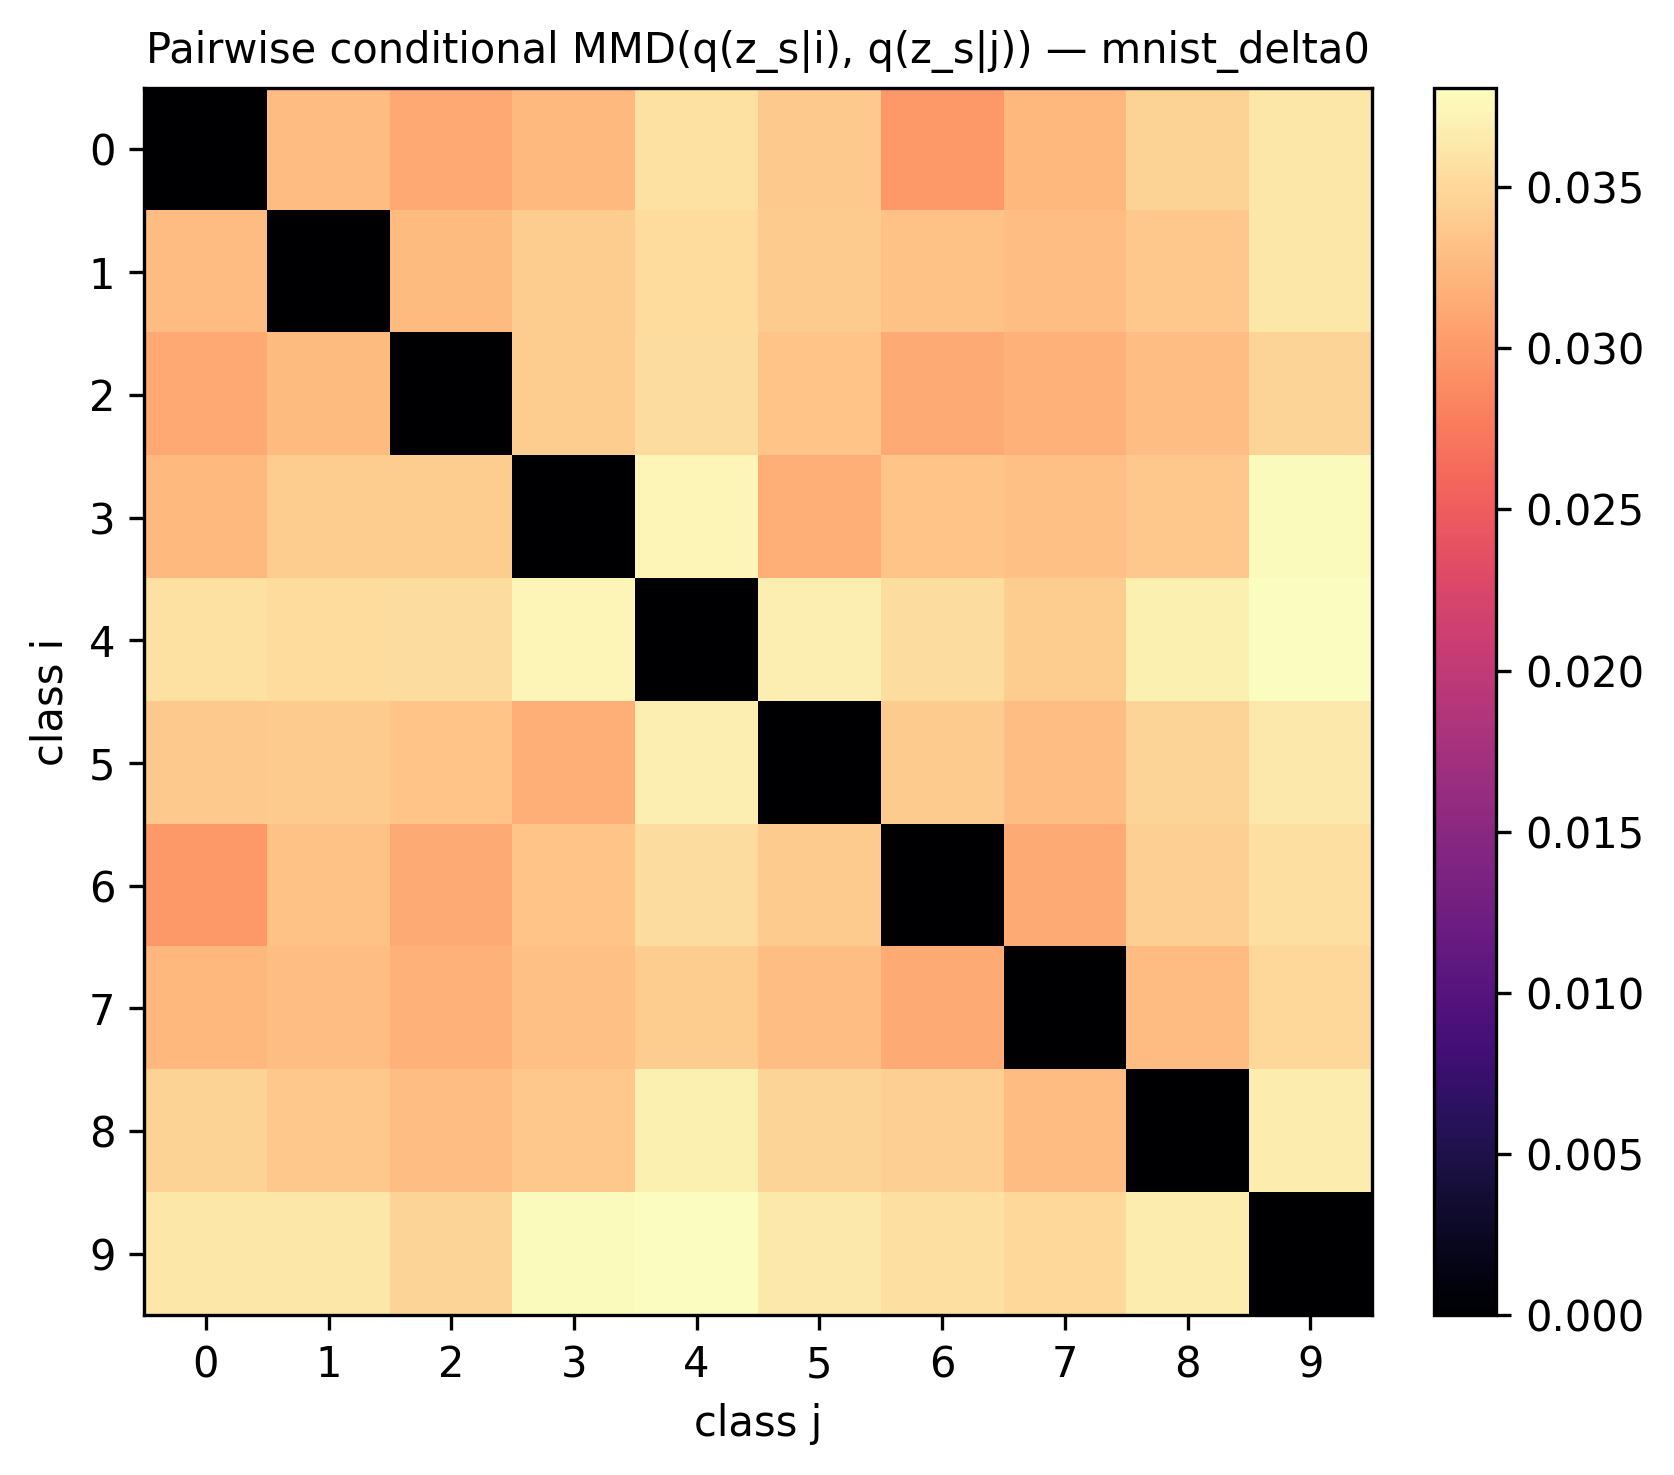
\includegraphics[width=\linewidth,trim=0 0 0 70,clip]{conditional_mmd_pairwise_heatmap_mnist.png}\\[-0.4em]
\small (a) MNIST
\end{minipage}\hfill
\begin{minipage}{0.47\textwidth}
\centering
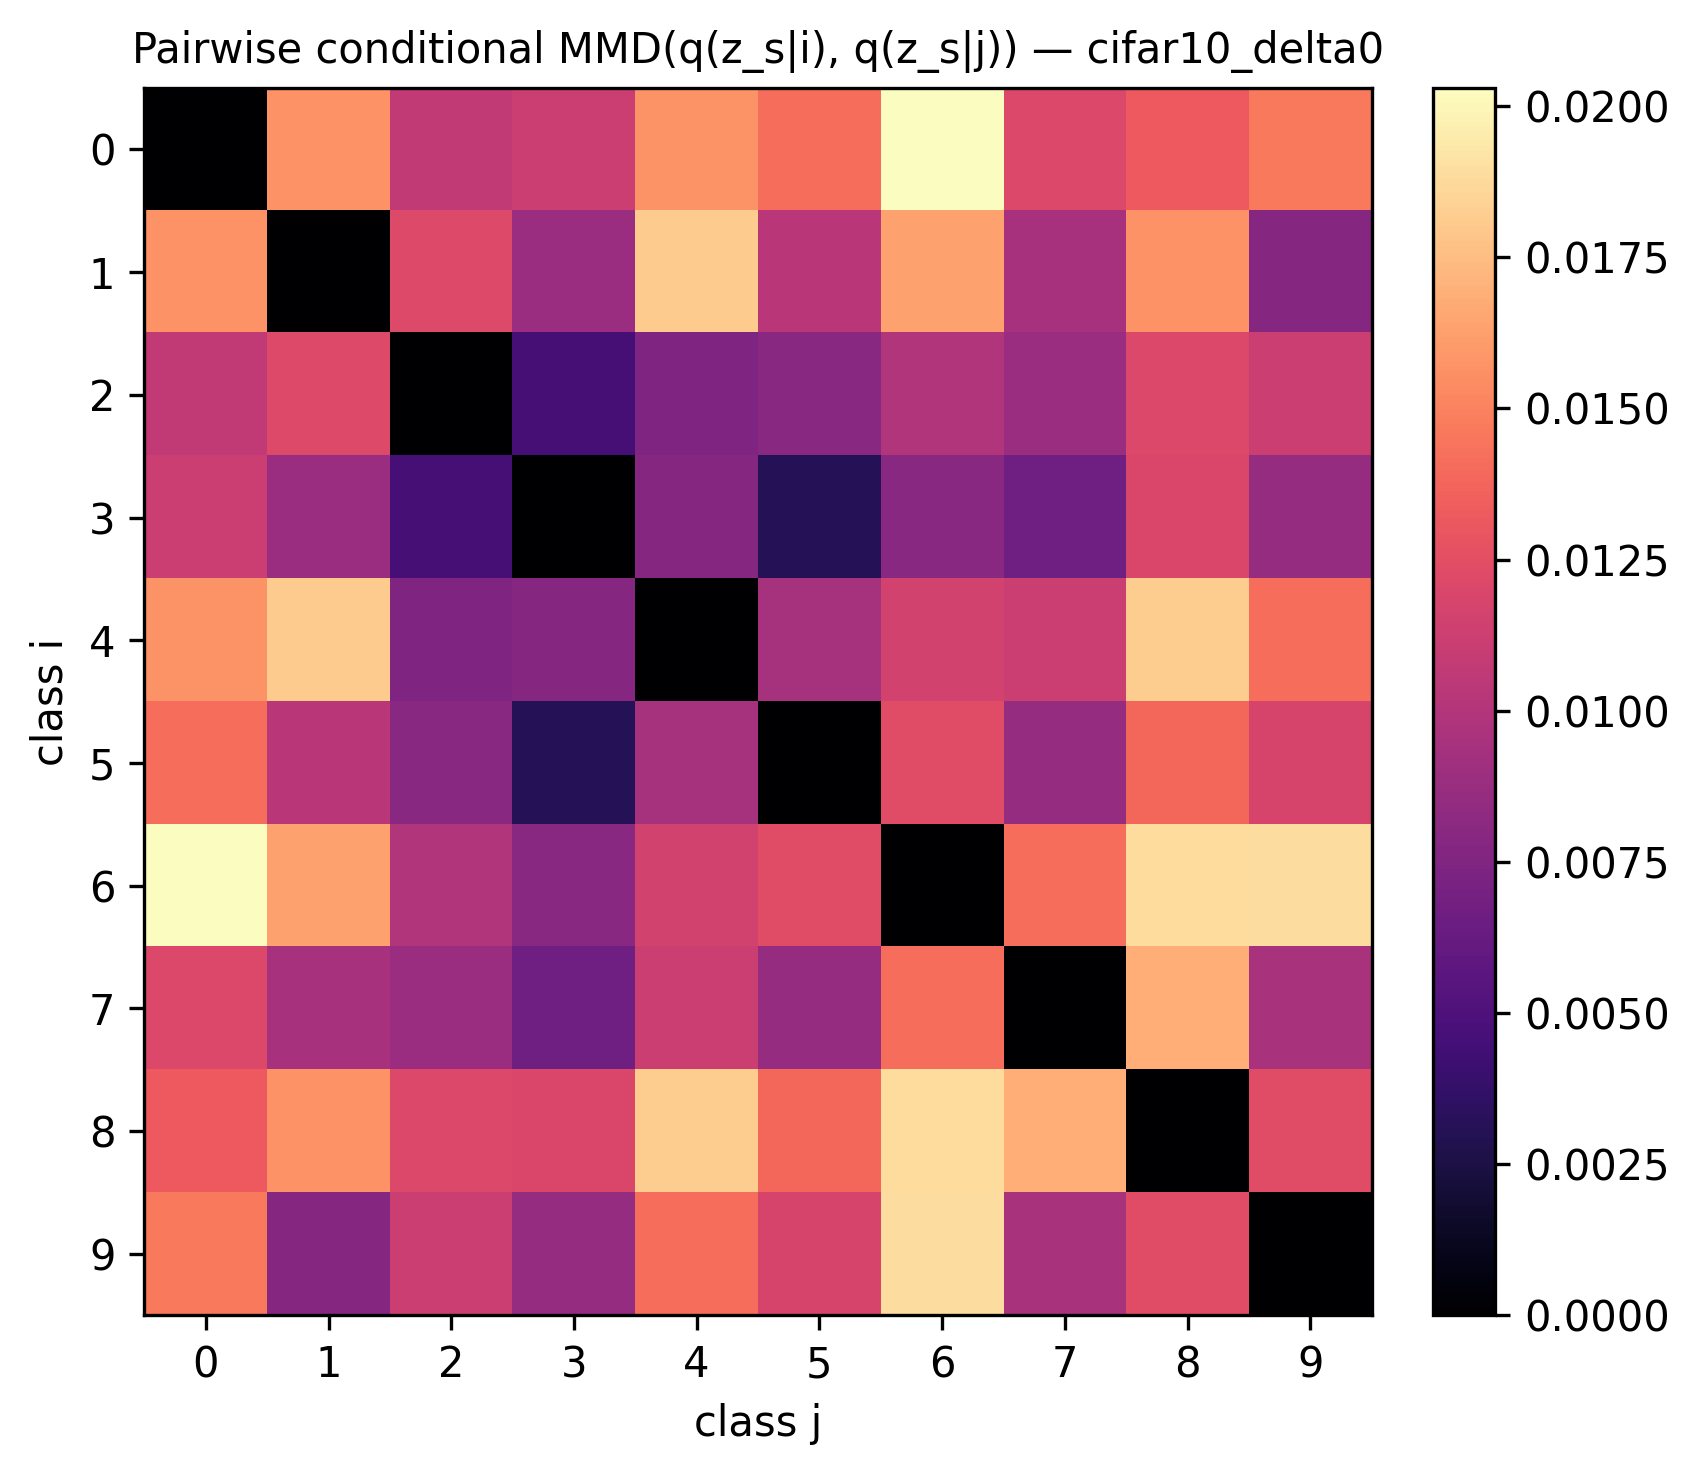
\includegraphics[width=\linewidth,trim=0 0 0 70,clip]{conditional_mmd_pairwise_heatmap_cifar10.png}\\[-0.4em]
\small (b) CIFAR-10
\end{minipage}
\caption{Pairwise $\MMD^2(q(\zs\mid y=i),q(\zs\mid y=j))$ for the
unrepaired seed-0 checkpoints.  The diagonal is zero by construction;
off-diagonal structure shows that conditional style distributions differ
throughout the label set.}
\label{fig:pairwise-mmd-app}
\end{figure}

Figure~\ref{fig:projection-app} gives a complementary one-dimensional view.
The projection direction is computed from the class means rather than chosen
after inspecting individual examples.  Several MNIST classes separate along
this direction, but the overlap also illustrates why a single projection is
not a substitute for the held-out multivariate probes.

\begin{figure}[t]
\centering
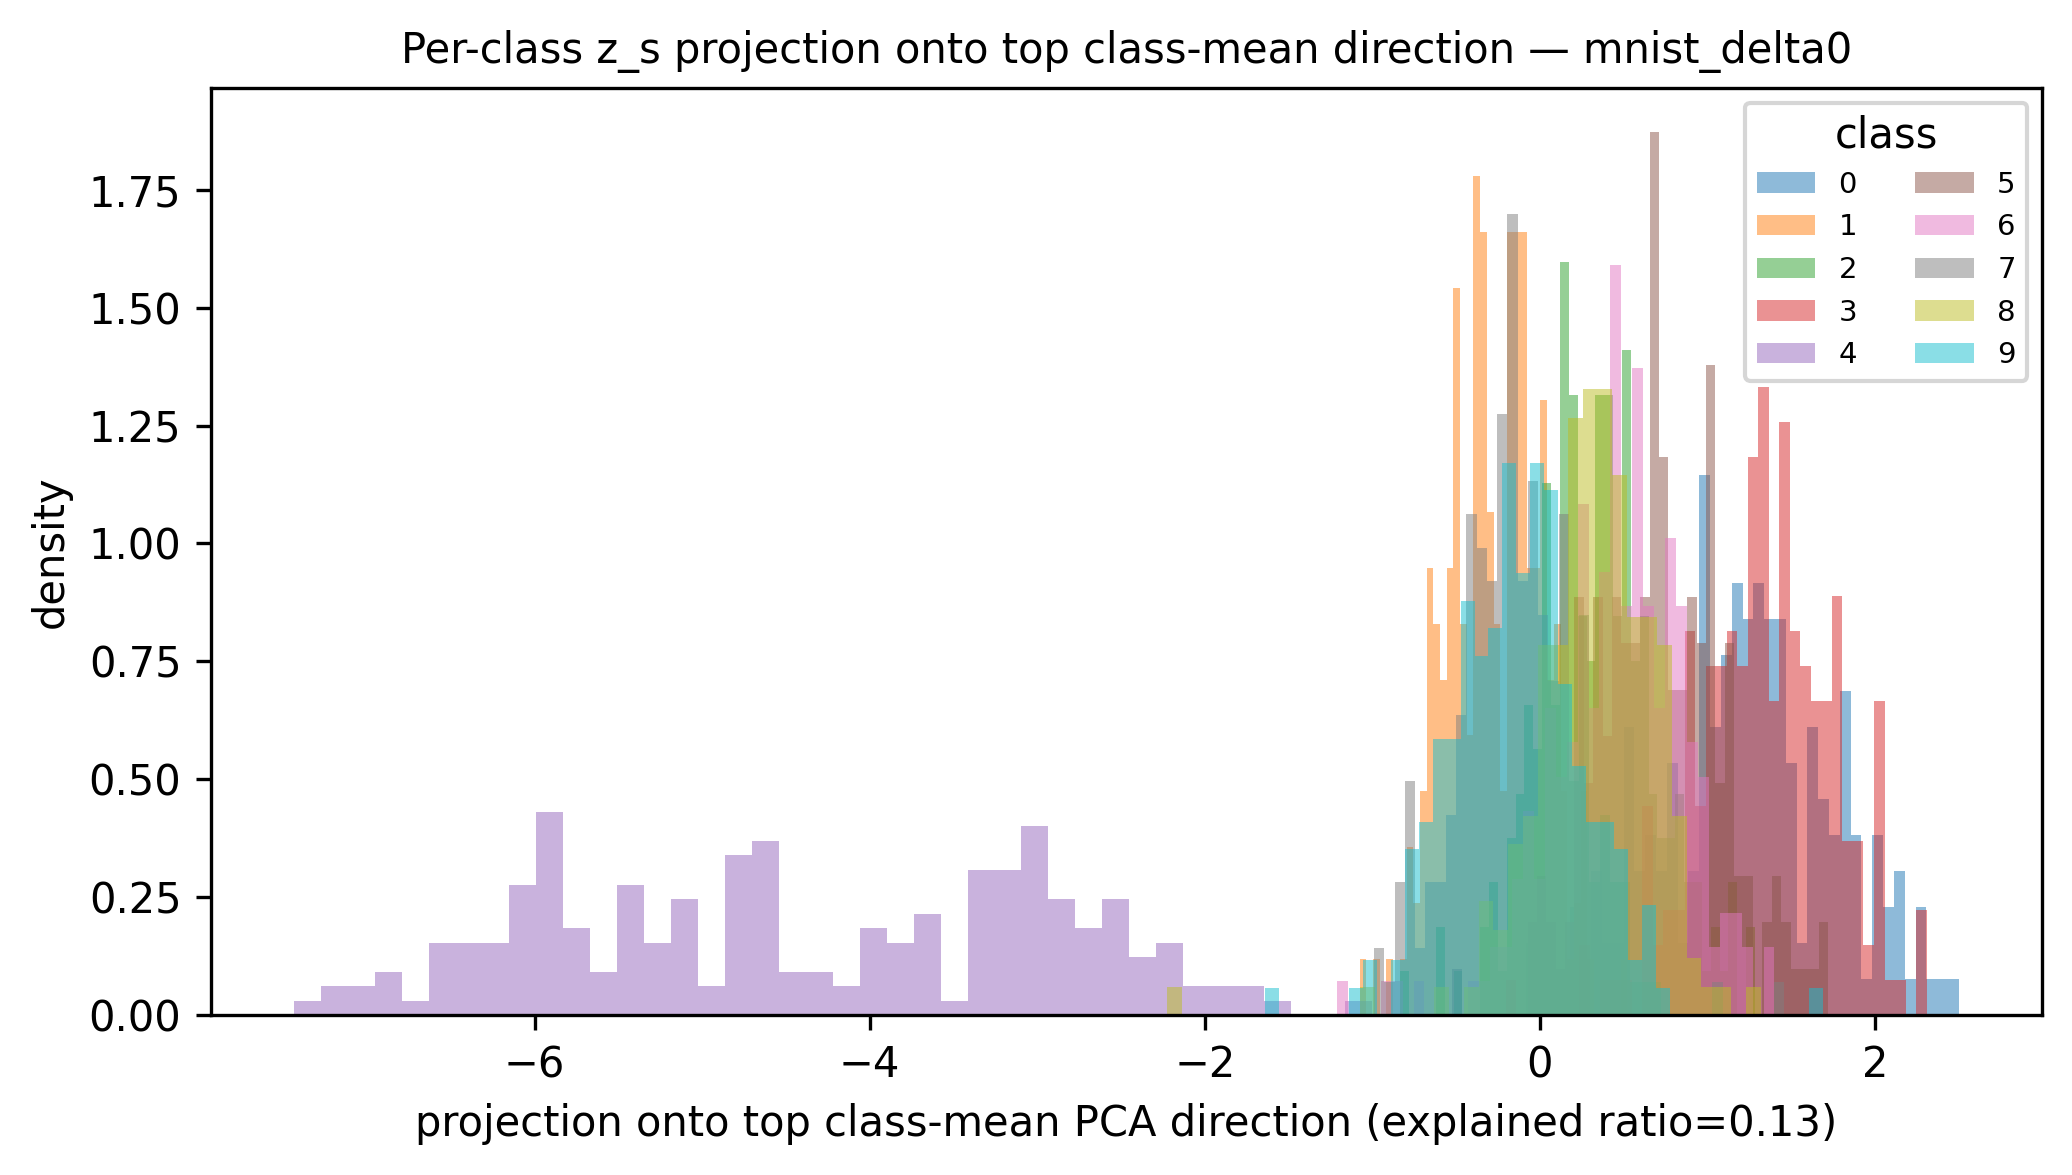
\includegraphics[width=0.78\textwidth,trim=0 0 0 80,clip]{conditional_mmd_projection_histogram_mnist.png}
\caption{MNIST stochastic styles projected onto the leading direction of
the class-mean matrix at $\delta=0$.  The direction explains 13.1\% of the
class-mean variance.  The plot is descriptive; the held-out probes and HSIC
tests provide the quantitative evidence.}
\label{fig:projection-app}
\end{figure}
\FloatBarrier

\subsection{Posterior-variance inspection}

The fractions of raw style log-variance coordinates at or below the clamp
floor are 99.9966\% (MNIST), 99.9989\% (Fashion-MNIST), and 100\% for all
three CIFAR-10 checkpoints.  Because this statistic was added during the
post-hoc checkpoint audit, it is reported in the human-readable audit report;
future manifests should also store it as a first-class numeric field.

\subsection{Complete conditional-regularization sweep}

Table~\ref{tab:full-delta-sweep} expands the four points shown in the main
paper to all six archived $\delta$ settings.  We retain ACC, $\Dinter$, and
FID because they are directly tied to the sweep artifacts, but omit the
historical probe column until it is regenerated with the canonical held-out
split.  Each point is a separate single-seed training run.

\begin{table}[ht]
\caption{Complete single-seed per-class-style-MMD sweep.  Lower FID and
$\Dinter$ are better; no uncertainty or significance claim is made.}
\label{tab:full-delta-sweep}
\centering
\small
\setlength{\tabcolsep}{4pt}
\begin{tabular}{lrrrrrr}
\toprule
& \multicolumn{3}{c}{MNIST} & \multicolumn{3}{c}{CIFAR-10} \\
$\delta$ & ACC & $\Dinter$ & FID & ACC & $\Dinter$ & FID \\
\midrule
0    & .9915 & 6.21 & 74.0 & .8129 & 3.74 & 80.5 \\
.03  & .9944 & 3.27 & 62.8 & .8111 & 2.48 & 79.1 \\
.1   & .9898 & 2.12 & 52.6 & .8100 & 2.03 & 77.5 \\
.3   & .9936 & 1.55 & 59.4 & .7148 & 1.59 & 72.0 \\
1    & .8592 & 1.22 & 43.4 & .8000 & 1.05 & 74.4 \\
3    & .9929 & 1.18 & 41.5 & .7994 & .95  & 76.1 \\
\bottomrule
\end{tabular}
\end{table}

\FloatBarrier

\section{Generation and Decoder Diagnostics}
\label{app:decoder}

\subsection{External generation evaluation}

The independent MNIST evaluator is a four-convolution CNN trained for 20
epochs on real images only.  Its standard test accuracy is 99.34\%.  The
CIFAR-10 evaluator is a WideResNet-28-10 trained for 200 epochs with standard
random-crop and horizontal-flip augmentation on real training images only;
its test accuracy is 96.16\%.  Neither evaluator contributes to the
generative model's loss.

\begin{table}[ht]
\caption{Per-checkpoint external Gen-ACC.  Each entry uses 1,000 images per
requested class and a class-conditional style bank fitted on 12,000 training
examples.}
\label{tab:generation-seeds}
\centering
\small
\begin{tabular}{llrr}
\toprule
Dataset & Model seed & Global Gaussian & Class diagonal $\tau=.25$ \\
\midrule
MNIST & 0 & 0.1047 & 1.0000 \\
CIFAR-10 & 0 & 0.1262 & 0.4016 \\
CIFAR-10 & 1 & 0.1320 & 0.5386 \\
CIFAR-10 & 2 & 0.1268 & 0.4747 \\
\bottomrule
\end{tabular}
\end{table}

The class-diagonal distribution is fit from encoded training styles and
therefore deliberately conditions style on the requested label.  Its gain
tests whether the decoder is sensitive to the conditional mismatch.  It is
not an unconditional generative model and does not repair the encoder.

Figure~\ref{fig:cifar-sampling-app} displays the qualitative counterpart of
Table~\ref{tab:generation-seeds}.  Conditioning style makes the requested
category more visually consistent in some rows, but shrinking the diagonal
Gaussian to $\tau=.25$ also reduces variation and can produce blurry or
prototype-like outputs.  This is why Gen-ACC is not interpreted as a
stand-alone measure of generative quality; diversity-sensitive evaluation on
the same generated pools remains necessary.

\begin{figure}[t]
\centering
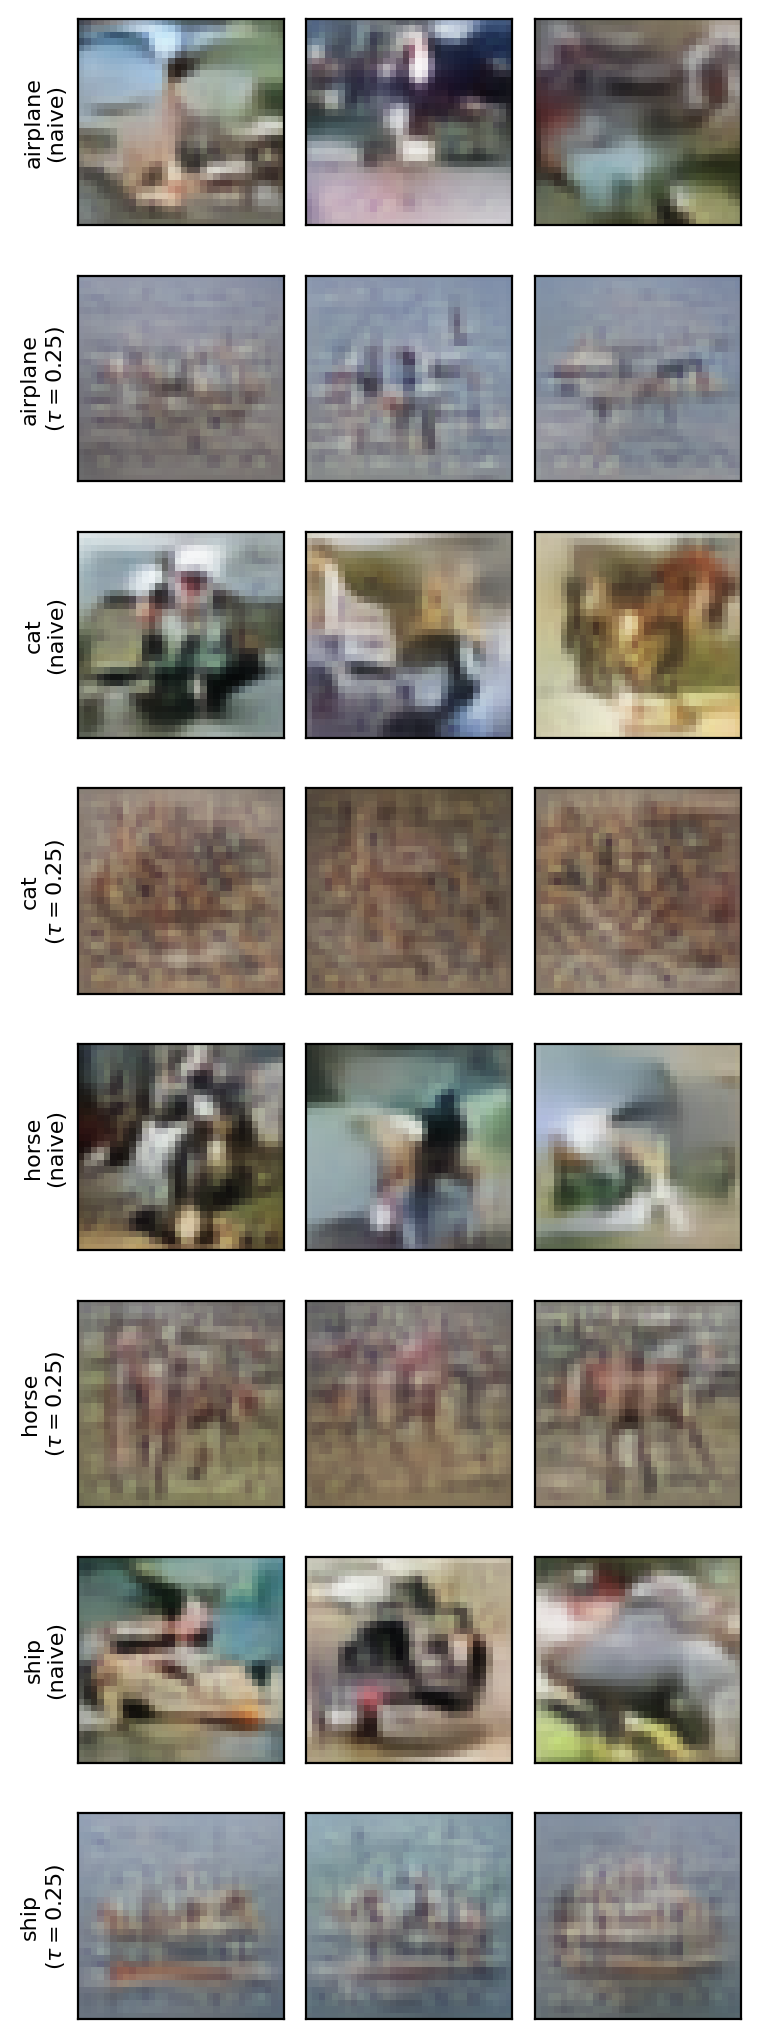
\includegraphics[width=0.43\textwidth]{cifar10_sampling_grid_trimmed.png}
\caption{Archived CIFAR-10 samples from the seed-0 checkpoint.  For four
requested classes, odd rows use the global Gaussian style prior and even rows
use the post-hoc class-diagonal prior at $\tau=.25$.  The grid is qualitative;
external Gen-ACC is reported in Table~\ref{tab:generation-seeds}.}
\label{fig:cifar-sampling-app}
\end{figure}
\FloatBarrier

\subsection{Independent-evaluator deterministic mean swaps}

For each ordered pair of distinct classes $(a,b)$, the diagnostic decodes
$\mathrm{Dec}(\muc^{(a)},\mus^{(b)})$ for 500 donor pairs and evaluates pixels
with the independent real-image classifier.  On unrepaired checkpoints,
identity follows the style donor on 99.28\% of MNIST and 63.92\% of CIFAR-10
off-diagonal swaps, while following the semantic donor on 0.06\% and 4.72\%.
At $\delta=1$, style-following falls to 23.37\% and 35.92\%, and semantic-
following rises to 51.00\% and 18.74\%, respectively.  Full rate matrices,
the other-class outcome, and pair-bootstrap intervals are stored in the
external-swap artifacts.

\begin{figure}[t]
\centering
\begin{minipage}{0.48\textwidth}
\centering
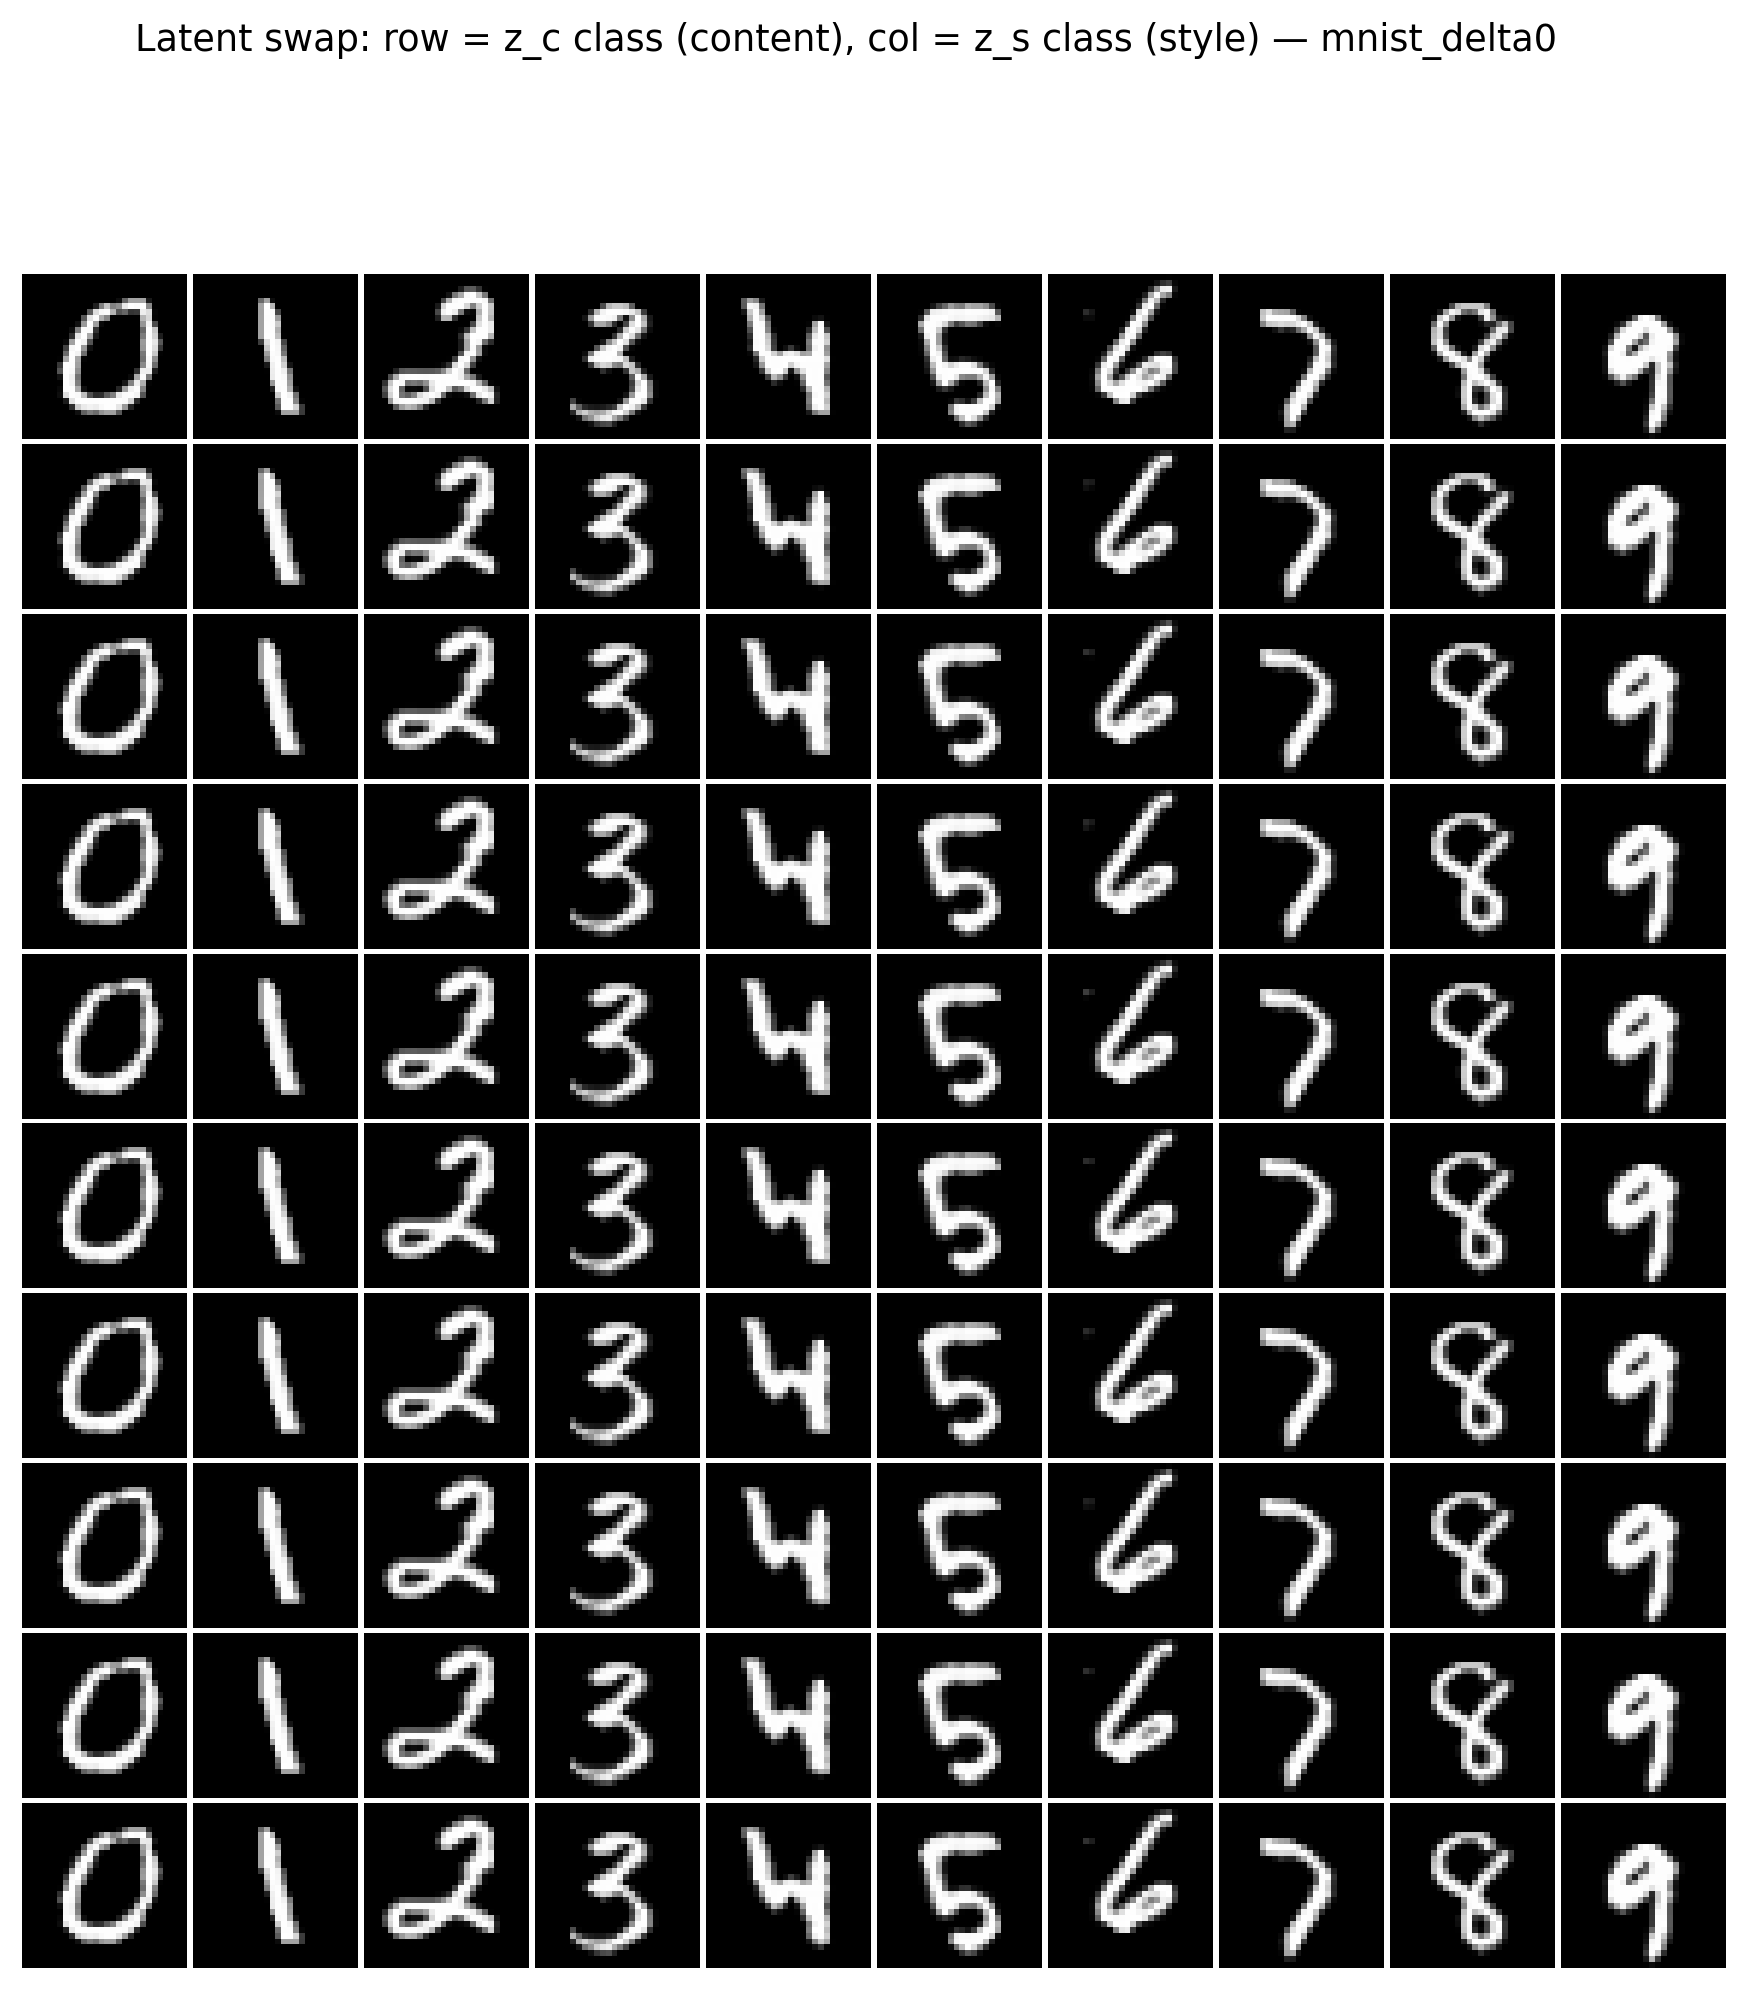
\includegraphics[width=0.86\linewidth]{mnist_swap_grid_delta0.png}\\[-0.4em]
\small (a) MNIST
\end{minipage}\hfill
\begin{minipage}{0.48\textwidth}
\centering
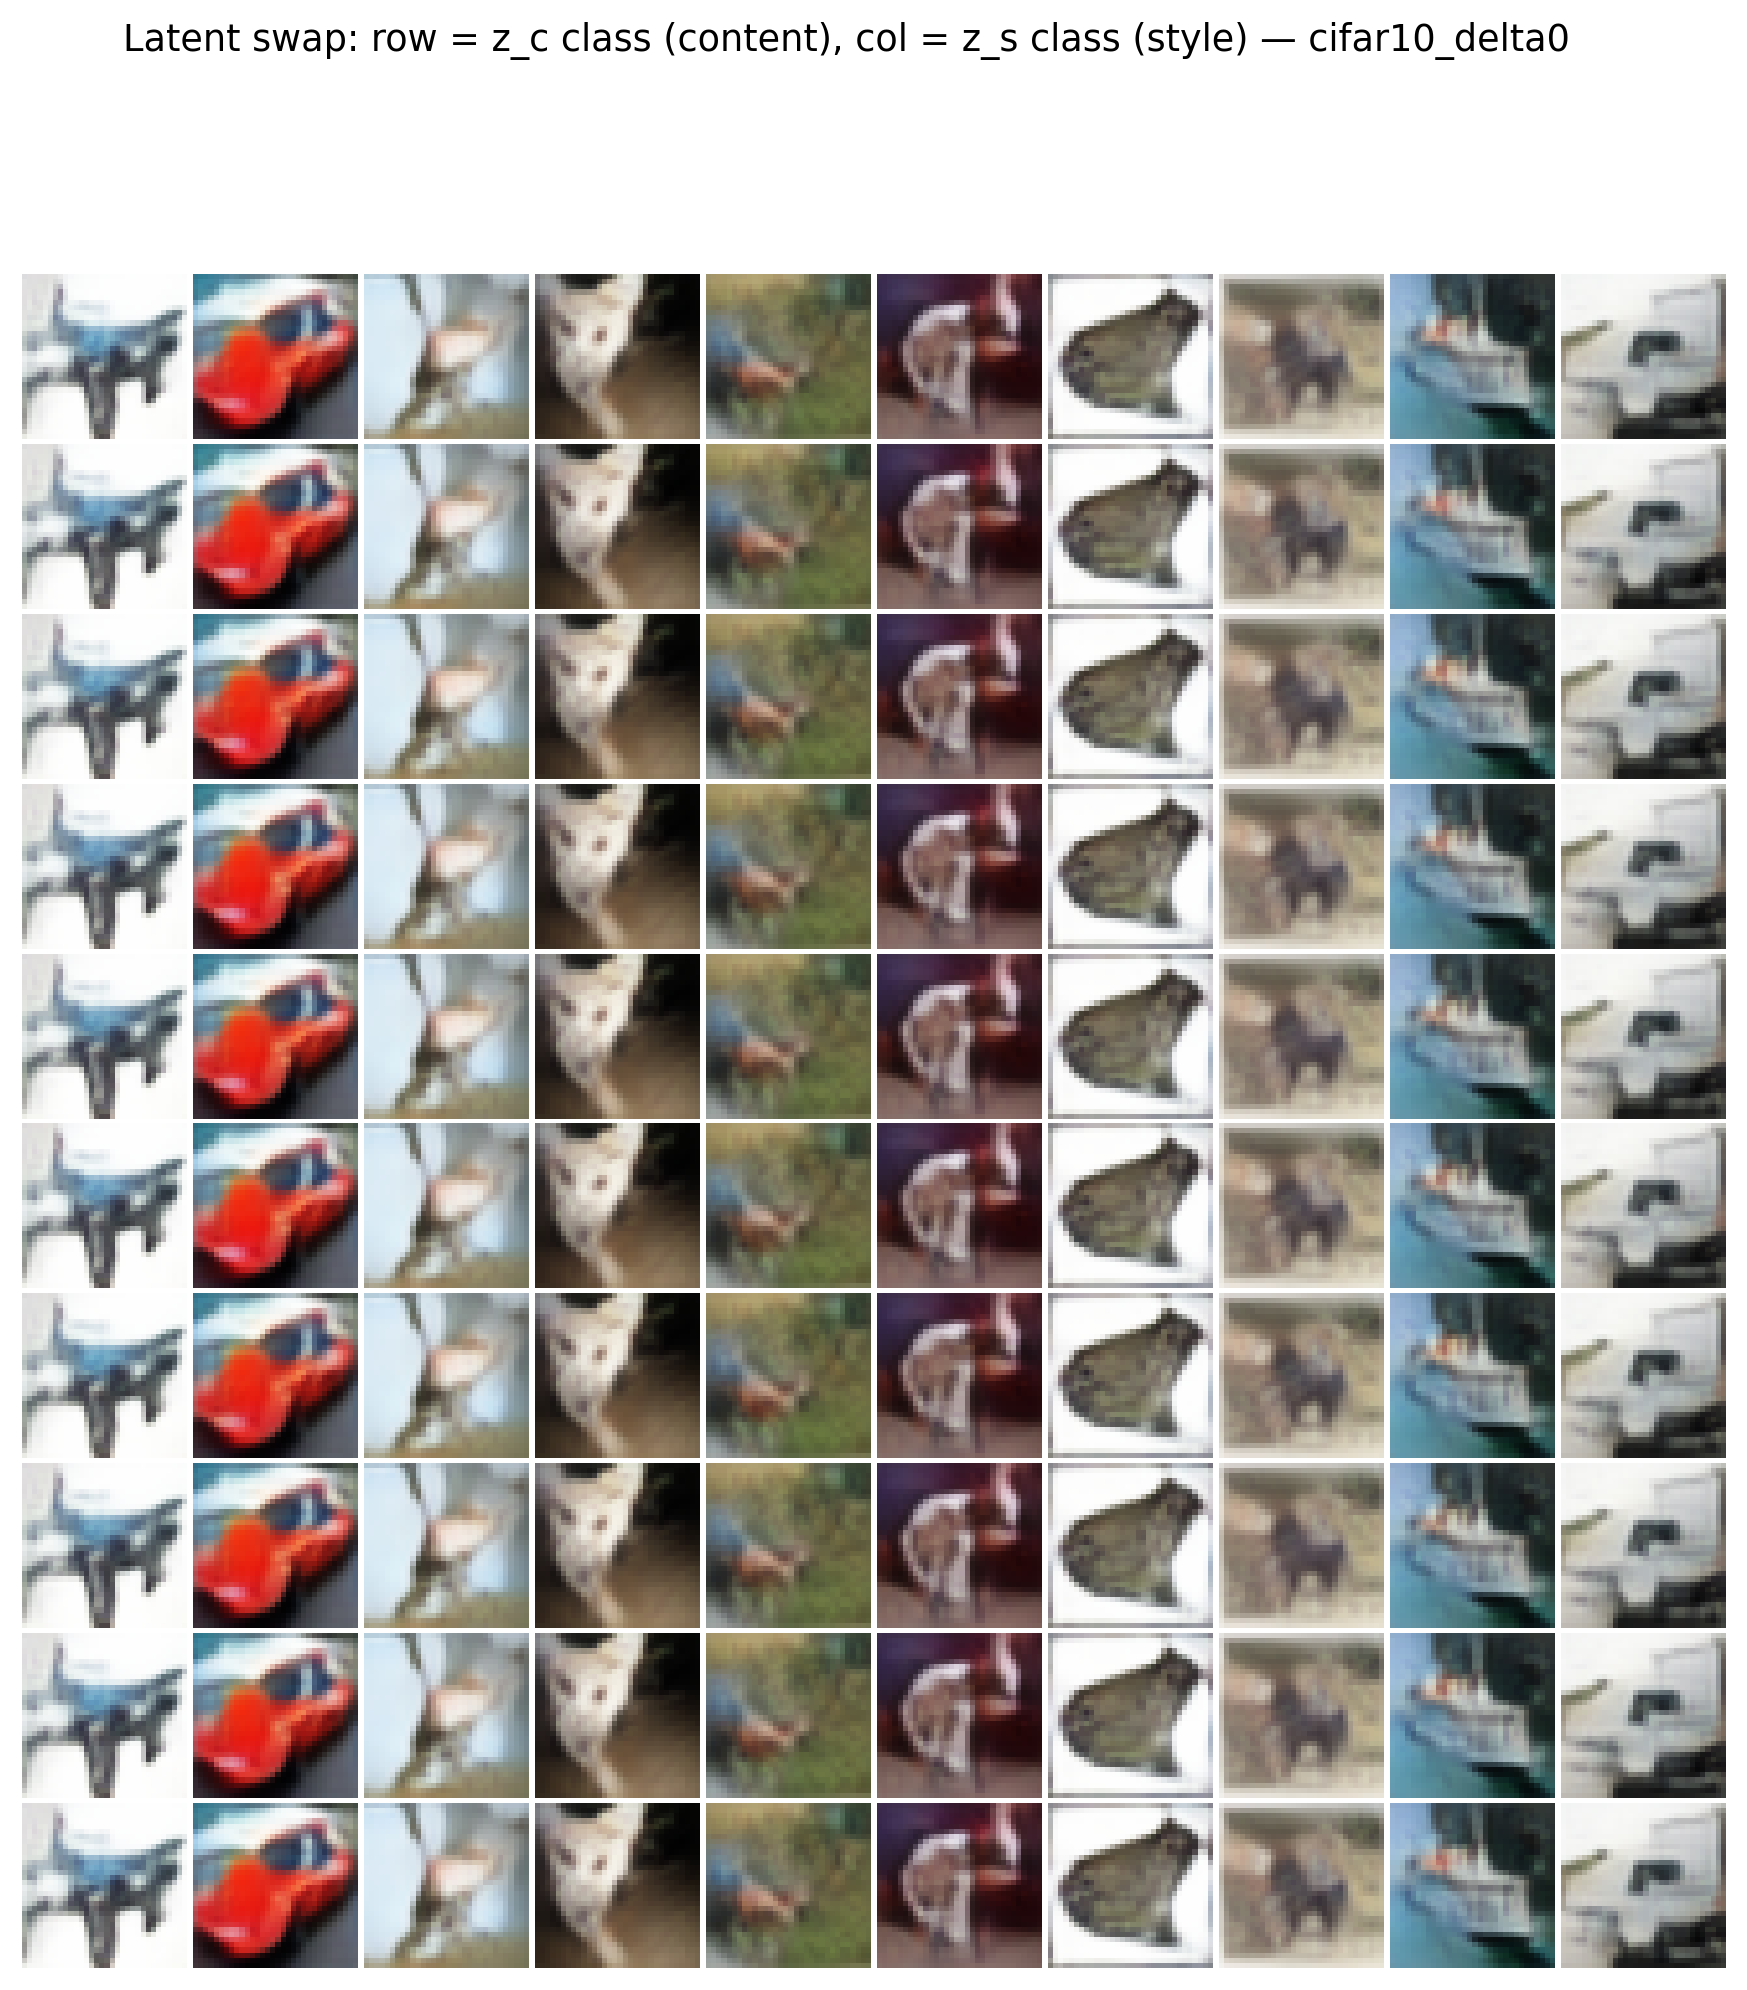
\includegraphics[width=0.86\linewidth]{cifar10_swap_grid_delta0.png}\\[-0.4em]
\small (b) CIFAR-10
\end{minipage}
\caption{Deterministic mean-swap grids at $\delta=0$.  Rows donate
semantic means and columns donate style means.  Column-controlled identity
is visually strong on MNIST and weaker but still present for several
CIFAR-10 classes.  Quantitative rates in the text use independent pixel
classifiers; the grids are qualitative.}
\label{fig:swap-grid-app}
\end{figure}
\FloatBarrier

\section{Reproducibility and Current Evidence Boundary}
\label{app:reproducibility-v8-superseded}

\iffalse % superseded by the v9 evidence boundary below

All Stage-0 results are stored as JSON plus SHA-256 sidecars.  Each manifest
records the repository state, checkpoint hash, evaluation seed, fixed subset,
latent view, probe split, feature preprocessing, and evaluator metadata.  The
canonical protocol version for the present draft is
\texttt{stage0-1.1.0}.  The five audited checkpoints are MNIST seed 0,
Fashion-MNIST seed 0, and CIFAR-10 seeds 0, 1, 2; all use evaluation seed 0.

The current draft intentionally excludes the earlier cross-model probe table,
multi-remedy comparison, five-seed remedy/sampling tables, and explicit
split-latent baseline ranges.  Those measurements were not yet regenerated
under the held-out Stage-0 protocol with complete artifacts.  They should be
reintroduced only after model-specific loaders, manifests, and canonical
outputs are available.  This boundary keeps every quantitative claim in the
present paper tied to an inspectable artifact.

The submission source, rendered author block, supplementary archive, and all
externally hosted materials must remain anonymous throughout review.
\fi

\section{Exact-Marginal Experiment}
\label{app:synthetic-v9}

\subsection{Construction and protocol}

For every replication we draw $n=2{,}048$ vectors
$z\sim\mathcal N(0,I_{128})$ once, then reuse that latent sample while drawing
binary labels from logits $[-\kappa z_1,\kappa z_1]$ for
$\kappa\in\{0,.5,1,2,4,8,16\}$.  Thus the population marginal and the
finite latent sample are invariant to $\kappa$; only the label mechanism
changes.  We run 50 replications from base seed 2027, 499 global-MMD
permutations, 499 HSIC permutations, and a stratified 60/20/20 linear-probe
split.  The independent Gaussian reference and the labels use distinct random
streams.  Plus-one calibration gives minimum $p=1/500$.

\begin{table}[ht]
\caption{Complete synthetic result.  Probe values are mean $\pm$ sample
standard deviation over 50 replications; rejection columns are empirical
rates.  The global statistic is repeated across $\kappa$ within each
replication by design.}
\label{tab:synthetic-full-v9}
\centering
\scriptsize
\setlength{\tabcolsep}{3.5pt}
\begin{tabular}{rrrrrrrr}
\toprule
$\kappa$ & Probe (\%) & $\widehat I_{LB}$ & Global MMD & MMD rej. & HSIC & HSIC rej. & Cond. MMD \\
\midrule
0   & $49.58\pm1.86$ & -.050 & $-9.47\!\times\!10^{-7}$ & .06 & .000176 & .02 & .000006 \\
.5  & $62.48\pm2.58$ & .031 & $-9.47\!\times\!10^{-7}$ & .06 & .000239 & 1.00 & .000130 \\
1   & $74.49\pm2.09$ & .171 & $-9.47\!\times\!10^{-7}$ & .06 & .000314 & 1.00 & .000280 \\
2   & $83.28\pm2.07$ & .334 & $-9.47\!\times\!10^{-7}$ & .06 & .000377 & 1.00 & .000405 \\
4   & $89.51\pm1.45$ & .437 & $-9.47\!\times\!10^{-7}$ & .06 & .000404 & 1.00 & .000455 \\
8   & $91.82\pm1.63$ & .471 & $-9.47\!\times\!10^{-7}$ & .06 & .000413 & 1.00 & .000479 \\
16  & $92.30\pm1.51$ & .475 & $-9.47\!\times\!10^{-7}$ & .06 & .000415 & 1.00 & .000478 \\
\bottomrule
\end{tabular}
\end{table}

The unbiased global MMD can be negative under the null.  Three of 50 global
tests reject, inside the frozen central 95\% prediction interval $[0,6]$ for
$\operatorname{Binomial}(50,.05)$.  HSIC has Spearman trend 1.0 and
conditional MMD trend .964.  Seven of eight frozen checks pass.  The failed
check required mean probe accuracy strictly above 90\% at each of
$\{4,8,16\}$; $\kappa=4$ reaches 89.51\%.  No threshold, level, or inequality
was changed after observing the result.

\begin{table}[ht]
\caption{Supplementary sample-size sensitivity at $\kappa=16$.  Values are
rounded aggregate results from the completed follow-up runs.}
\label{tab:synthetic-n-v9}
\centering
\small
\begin{tabular}{rrr}
\toprule
$n$ & Probe accuracy (\%) & Global-MMD rejection (\%) \\
\midrule
512  & 92.0 & 6.0 \\
1,024 & 92.2 & 5.0 \\
2,048 & 92.3 & 6.0 \\
4,096 & 92.5 & 5.0 \\
\bottomrule
\end{tabular}
\end{table}

The probe effect is essentially stable across an eightfold range in sample
size, whereas the rejection rate remains near the nominal $5\%$ level.  The
follow-up therefore supports a variance-reduction interpretation rather than
an effect-size increase with $n$.

\section{Controlled Posterior-Entropy Intervention}
\label{app:entropy-v9}

The intervention adds a fixed floor in variance space and uses the resulting
$\sigma_{\rm eff}$ in both training and audit.  A floor of zero reproduces the
historical sampler.  Every nonzero setting is retrained for 300 epochs with
MNIST model seed 0 and CIFAR-10 model seeds $\{0,1,2\}$; the corresponding
baseline checkpoints are reused.  The CIFAR-10 confirmation
levels $\{0,.15,.35\}$ were fixed after both $.15$ and $.35$ passed the
predeclared MNIST promotion rule.  That rule required an entropy increase of
at least .75 nats/dimension, probe accuracy at least .20, HSIC rejection,
conditional MMD above global MMD, and final reconstruction no more than twice
baseline.

\begin{table}[ht]
\caption{Complete MNIST entropy sweep.  Median standard deviation is the
effective posterior value; floor hit refers to the raw log-variance head.}
\label{tab:entropy-mnist-full-v9}
\centering
\scriptsize
\setlength{\tabcolsep}{3.2pt}
\resizebox{\textwidth}{!}{%
\begin{tabular}{rrrrrrrrrrr}
\toprule
$\sigma_f$ & $H$/dim & Med. std & Raw floor & Probe & $\widehat I_{LB}$ & Global & Cond. & Ratio & Gen-ACC & Rec. \\
\midrule
0 & -3.581 & .00674 & 100.00\% & 99.76\% & 2.283 & .000579 & .016024 & 27.68 & 10.15\% & .01259 \\
.025 & -2.215 & .02589 & 99.16\% & 99.51\% & 2.273 & .000599 & .016352 & 27.31 & 10.05\% & .01273 \\
.05 & -1.553 & .05045 & 99.17\% & 99.51\% & 2.273 & .000648 & .016135 & 24.88 & 11.95\% & .01315 \\
.15 & -.477 & .15015 & 99.77\% & 98.78\% & 2.228 & .000654 & .012044 & 18.41 & 37.35\% & .01520 \\
.35 & .381 & .35006 & 96.50\% & 95.61\% & 2.159 & .000518 & .007516 & 14.51 & 93.50\% & .01658 \\
\bottomrule
\end{tabular}}
\end{table}

\begin{table}[ht]
\caption{Seed-0 detail for the fixed CIFAR-10 entropy confirmation.}
\label{tab:entropy-cifar-full-v9}
\centering
\scriptsize
\setlength{\tabcolsep}{3.2pt}
\begin{tabular}{rrrrrrrrrr}
\toprule
$\sigma_f$ & $H$/dim & Med. std & Probe & $\widehat I_{LB}$ & Global & Cond. & Ratio & Gen-ACC & Rec. \\
\midrule
0 & -3.581 & .00674 & 61.46\% & 1.111 & .000249 & .005789 & 23.29 & 12.60\% & .05140 \\
.15 & -.477 & .15015 & 28.78\% & .256 & .000743 & .003690 & 4.97 & 27.35\% & .05940 \\
.35 & .369 & .35006 & 9.76\% & -.115 & .000667 & .001287 & 1.93 & 54.25\% & .06476 \\
\bottomrule
\end{tabular}
\end{table}

\begin{table}[ht]
\caption{Three-seed CIFAR-10 entropy confirmation.  Entries are rounded means
over model seeds; $p=.00498$ means that every seed reaches the minimum
plus-one calibrated HSIC value with 200 permutations.}
\label{tab:entropy-cifar-aggregate-v9}
\centering
\scriptsize
\setlength{\tabcolsep}{4pt}
\begin{tabular}{rrrrrrr}
\toprule
$\sigma_f$ & Probe (\%) & Global MMD & Cond. MMD & HSIC $p$ & Gen-ACC (\%) & Rec. L1 \\
\midrule
0 & 68.0 & .00030 & .0058 & .00498 & 13.0 & .052 \\
.15 & 29.0 & .00070 & .0037 & .00498 & 27.0 & .059 \\
.35 & 10.5 & .00067 & .0013 & .00498 & 52.0 & .065 \\
\bottomrule
\end{tabular}
\end{table}

HSIC attains $p=1/201$ at every MNIST level and for every CIFAR-10 seed.  This
outcome is read alongside effect sizes: the three-seed CIFAR-10 $.35$ probe is
only $10.5\%$ and does not support practically recoverable label information
even though the kernel test still detects dependence.  Raw floor-hit is 100\%
at all CIFAR levels;
the experiment manipulates effective noise rather than claiming that the
variance head stops collapsing.

\begin{figure}[ht]
\centering
\begin{minipage}{0.49\textwidth}
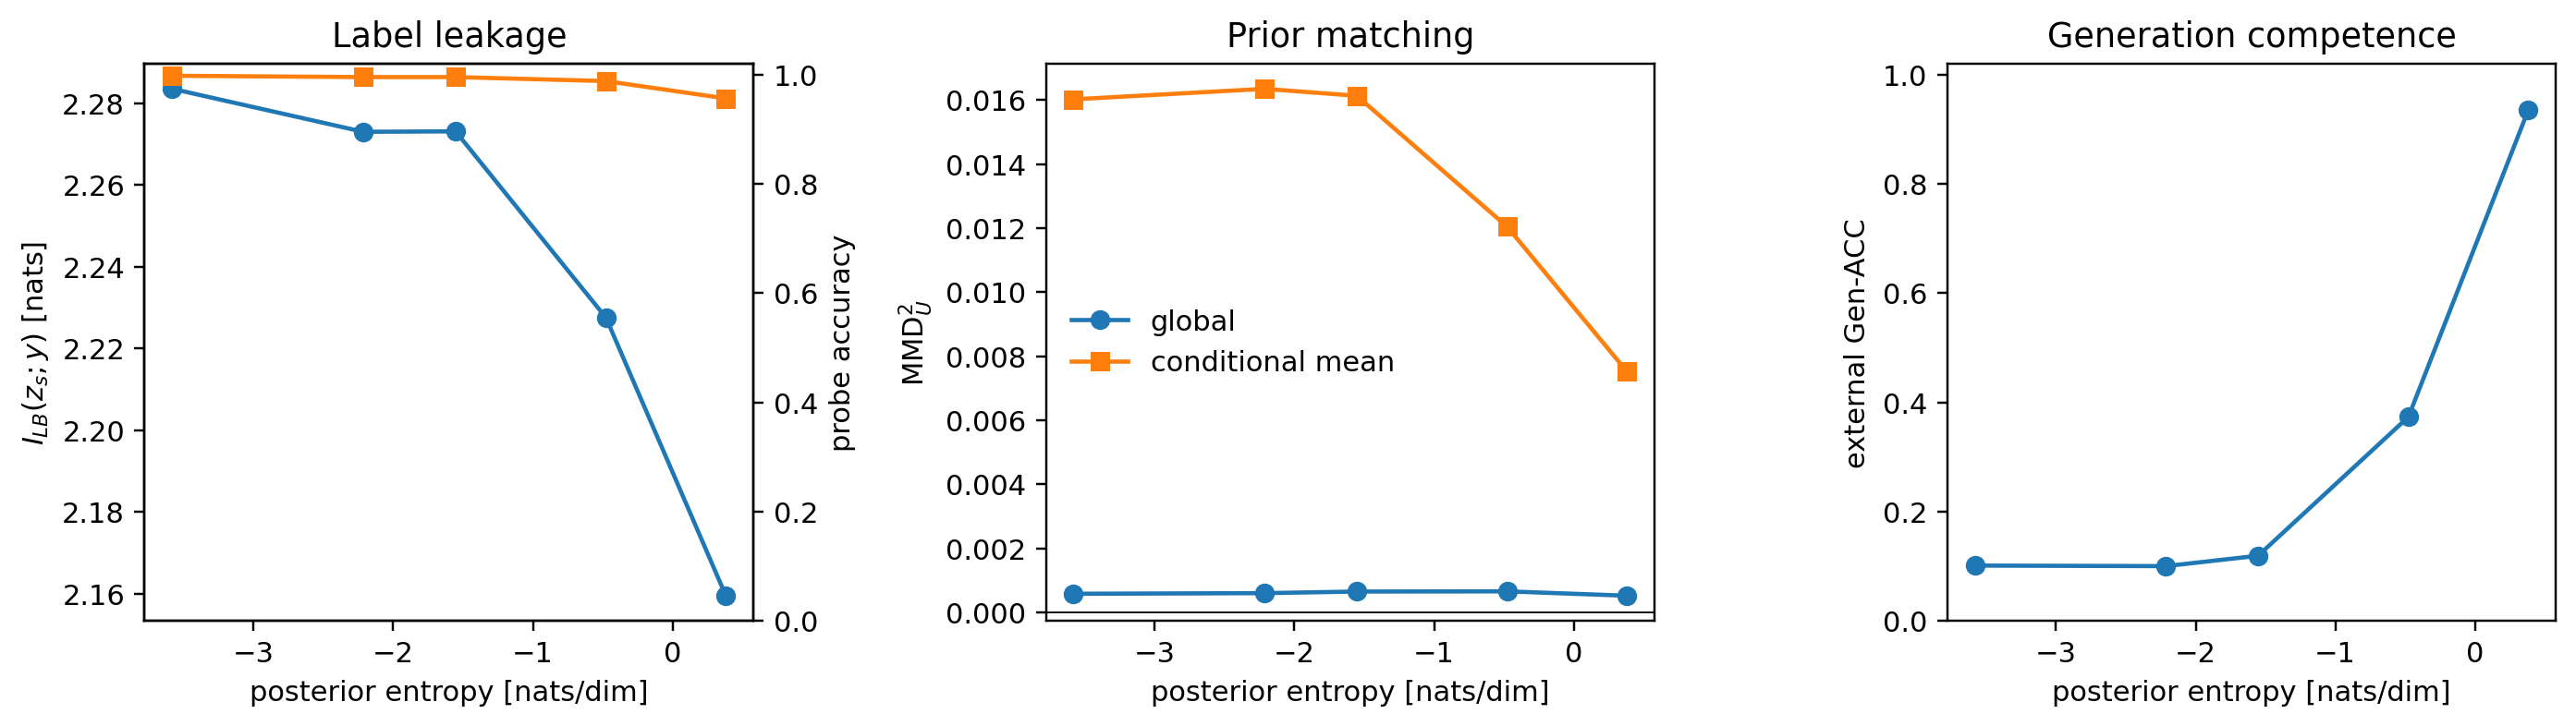
\includegraphics[width=\linewidth]{entropy_sweep_mnist.png}\\[-0.4em]
\centering\small (a) MNIST
\end{minipage}\hfill
\begin{minipage}{0.49\textwidth}
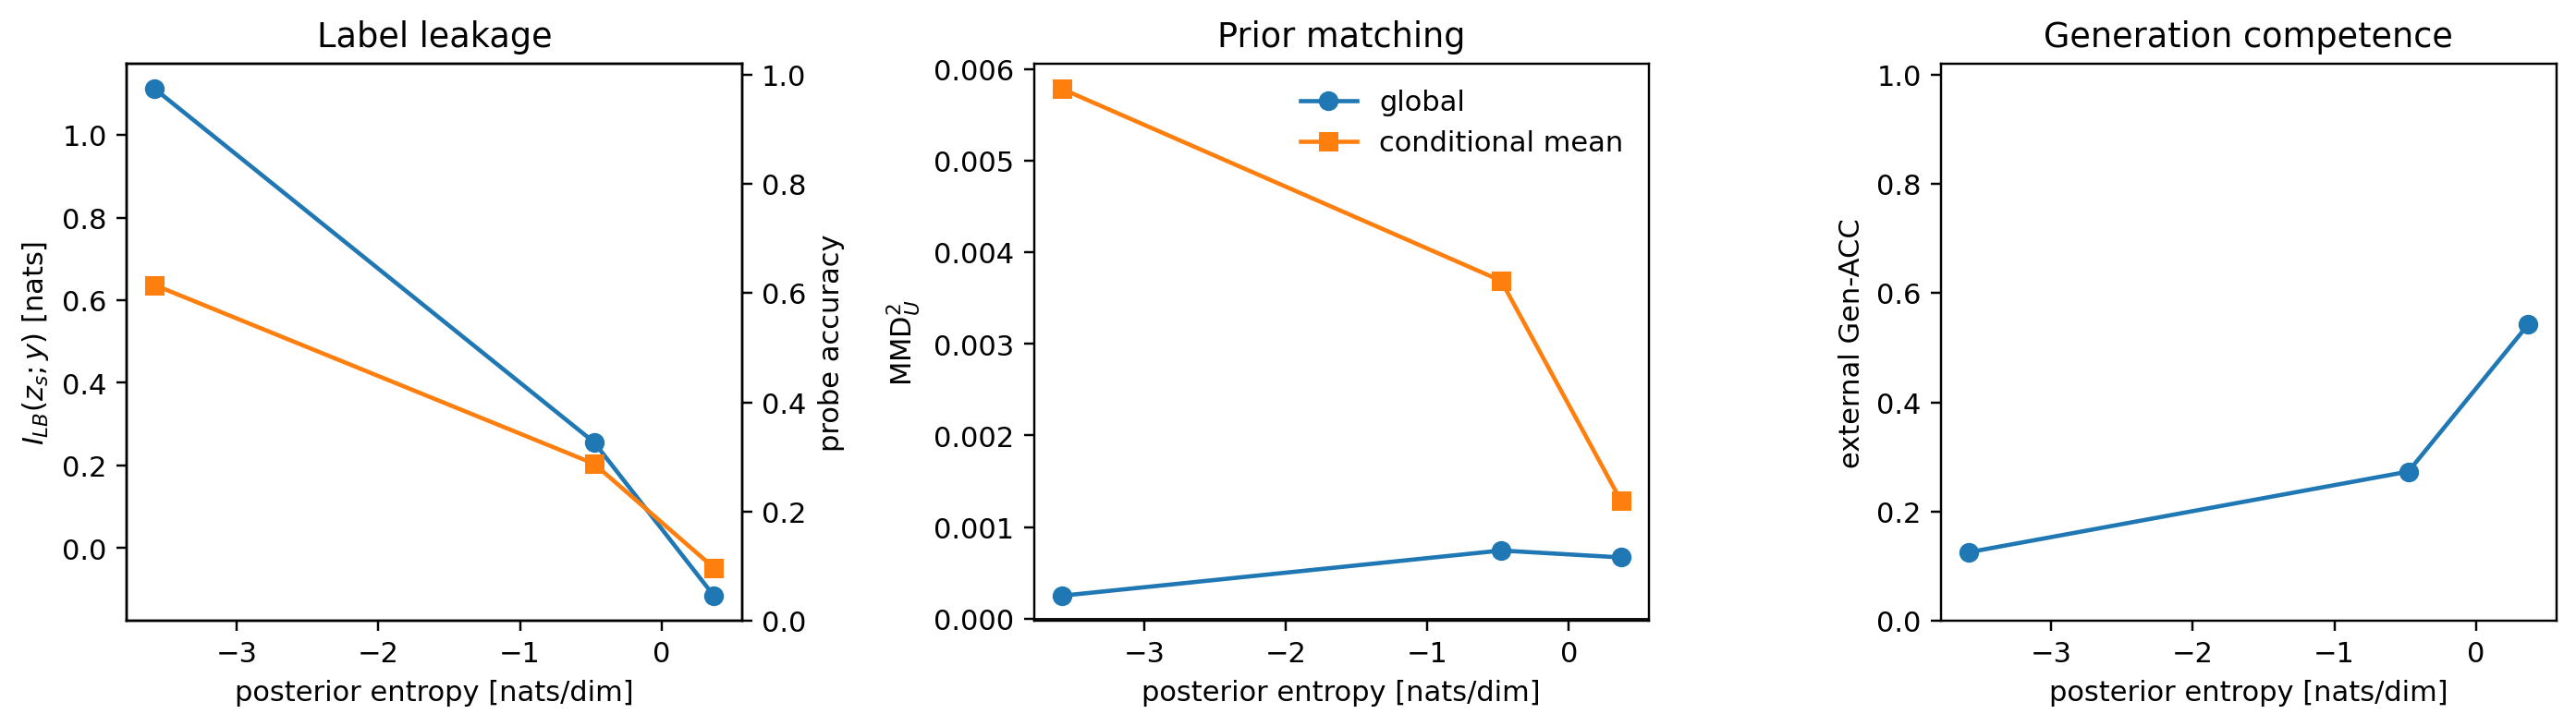
\includegraphics[width=\linewidth]{entropy_sweep_cifar10.png}\\[-0.4em]
\centering\small (b) CIFAR-10
\end{minipage}
\caption{Leakage, marginal/conditional discrepancy, and independent Gen-ACC
as effective posterior entropy increases.  Curves are single-seed controlled
interventions, not confidence intervals over training.}
\label{fig:entropy-full-v9}
\end{figure}
\FloatBarrier

\section{Native Cross-Model Details}
\label{app:cross-model-v9}

The fixed population contains 40,000 paired training examples and 10,000
paired test examples.  Each canonical domain audit uses 1,000 balanced test
examples.  The independent Rotated-MNIST evaluator is trained only on real
images and reaches 96.05\% test accuracy.  All models use their final
100-epoch checkpoint for seeds 0--2.

\begin{table}[ht]
\caption{Per-seed native cross-model results, macro-averaged over the two
domains.  Probe, content, and retention values are percentages.}
\label{tab:cross-model-seeds-v9}
\centering
\scriptsize
\setlength{\tabcolsep}{3pt}
\resizebox{\textwidth}{!}{%
\begin{tabular}{llrrrrrrr}
\toprule
Family & Seed & Global & Cond. & Logit & RBF & HSIC domains & Content & Retention \\
\midrule
F-CS-WAE & 0 & .003287 & .032431 & 94.00 & 97.75 & 2/2 reject & 99.25 & 12.55 \\
F-CS-WAE & 1 & .003209 & .030989 & 92.50 & 96.25 & 2/2 reject & 99.50 & 11.10 \\
F-CS-WAE & 2 & .003481 & .033365 & 89.25 & 96.00 & 2/2 reject & 99.50 & 13.45 \\
\midrule
DRIT & 0 & .259014 & .272479 & 25.00 & 25.50 & 2/2 reject & 87.50 & 9.80 \\
DRIT & 1 & .261287 & .274362 & 29.50 & 23.25 & 2/2 reject & 90.00 & 10.00 \\
DRIT & 2 & .245482 & .270487 & 48.75 & 48.75 & 2/2 reject & 87.25 & 9.80 \\
\midrule
DIVA & 0 & .0000096 & .000268 & 11.50 & 12.50 & .0746, .0398 & 96.00 & 90.25 \\
DIVA & 1 & -.0000452 & .0000288 & 11.00 & 11.25 & .2687, .0249 & 97.50 & 89.50 \\
DIVA & 2 & -.0000181 & .000231 & 9.50 & 11.75 & .1194, .7264 & 96.50 & 88.60 \\
\bottomrule
\end{tabular}}
\end{table}

All F-CS-WAE and DRIT domain-level HSIC values equal $1/201$.  For DIVA, Holm
step-down correction over its six raw tests leaves no rejection.  DIVA's six
global-MMD tests also do not reject.  Its posterior entropy is approximately
1.36--1.38 nats/dimension; F-CS-WAE is approximately -3.58 and DRIT ranges
from -1.88 to -1.57.  The cross-model result therefore does not by itself
remove posterior entropy as a confound for F-CS-WAE; that role belongs to
Appendix~\ref{app:entropy-v9}.

\section{Shapes3D Known-Factor Audit}
\label{app:shapes3d-v9}

Shapes3D provides 480,000 $64\times64$ images containing every combination of
10 floor hues, 10 wall hues, 10 object hues, 8 scales, 4 shapes, and 15
orientations.  The fixed shape-stratified IID split contains 120,000 training,
20,000 validation, and 20,000 test images.  F-CS-WAE and the learned C/S VAE
use seeds $\{0,1,2\}$; the observed-shape oracle uses seed 0.  Every model has
64 content and 64 style dimensions and is audited at epoch 100 on 4,096
examples (1,024 per shape).  Global MMD uses 2,048 examples and 500
permutations; factor HSIC uses
up to 1,024 examples and 200 permutations.  Holm correction is applied
separately within each latent view.

\begin{table}[ht]
\caption{Completed three-seed Shapes3D replication.  Entries are rounded
means over seeds $\{0,1,2\}$.  The observed-shape oracle remains a seed-0
auxiliary control and is reported in the main paper.}
\label{tab:shapes3d-aggregate-v9}
\centering
\scriptsize
\setlength{\tabcolsep}{3.5pt}
\resizebox{\textwidth}{!}{%
\begin{tabular}{lrrrrrr}
\toprule
Model & $z_s\!\to$shape & $z_c\!\to$style & Cond. shape MMD & Prior shape & Swap shape & Rec. L1 \\
\midrule
F-CS-WAE & 99.0 & 87.0 & .0085 & 89.0 & 88.0 & .0023 \\
Learned C/S VAE & 25.5 & 9.5 & .00004 & 99.7 & 99.8 & .0029 \\
\bottomrule
\end{tabular}}
\end{table}

\begin{table}[ht]
\caption{Seed-0 held-out logistic factor probes on stochastic latent samples.
Columns follow dataset order.  The intended pattern is content high only for
shape and style low only for shape.}
\label{tab:shapes3d-probes-full-v9}
\centering
\scriptsize
\setlength{\tabcolsep}{3pt}
\resizebox{\textwidth}{!}{%
\begin{tabular}{lllrrrrrr}
\toprule
Model & View & Floor & Wall & Object & Scale & Shape & Orient. \\
\midrule
F-CS-WAE & content & 99.76 & 99.88 & 80.98 & 68.05 & 100.00 & 89.88 \\
          & style   & 100.00 & 100.00 & 100.00 & 95.61 & 100.00 & 100.00 \\
\midrule
Observed-shape cVAE & content & 9.76 & 9.51 & 9.02 & 14.27 & 100.00 & 8.29 \\
                    & style   & 100.00 & 99.63 & 99.02 & 45.49 & 25.98 & 39.76 \\
\midrule
Learned C/S VAE & content & 8.90 & 11.22 & 8.90 & 11.95 & 100.00 & 5.85 \\
                & style   & 84.02 & 91.46 & 88.29 & 44.15 & 25.73 & 42.93 \\
\bottomrule
\end{tabular}}
\end{table}

After Holm correction, F-CS-WAE rejects dependence for all six factors in
both views.  Each control rejects only shape in content and only the five
nuisance factors in style.  The corresponding shape HSIC raw $p$-values in
style are .597 for the observed-shape cVAE and .826 for the learned model.

\begin{table}[ht]
\caption{Seed-0 independent factor-evaluator decoder checks.  Posterior swaps keep
content from the source and style from a different-shape donor; ``target'' is
source shape for shape and donor value for nuisance factors.}
\label{tab:shapes3d-decoder-full-v9}
\centering
\scriptsize
\setlength{\tabcolsep}{3pt}
\resizebox{\textwidth}{!}{%
\begin{tabular}{lrrrrrrr}
\toprule
Model & Floor & Wall & Object & Scale & Orient. & Swap shape & Prior shape \\
\midrule
F-CS-WAE & 100.00 & 99.90 & 99.95 & 80.93 & 100.00 & 87.74 & 89.43 \\
Observed-shape cVAE & 99.98 & 100.00 & 99.80 & 95.02 & 99.93 & 100.00 & 99.88 \\
Learned C/S VAE & 99.98 & 99.93 & 99.85 & 99.73 & 99.93 & 100.00 & 99.78 \\
\bottomrule
\end{tabular}}
\end{table}

All three models pass the frozen competence checks: independent factor
evaluator, content-shape probe, reconstruction L1 below .12, reconstruction
shape accuracy above .8, and mean reconstructed nuisance-factor accuracy
above .7.  The observed-shape cVAE supplies content directly from the label;
it is an oracle control for the intended split, not a like-for-like
representation-learning competitor.  The learned content--style VAE is the
stronger negative control.

\section{Reproducibility and Evidence Boundary}
\label{app:reproducibility}

The original checkpoint audit uses protocol \texttt{stage0-1.1.0}; all new
synthetic, entropy, cross-model, and Shapes3D audits use
\texttt{stage0-1.2.0}.  Primary artifact roots are:
\begin{itemize}
    \item \texttt{runs\_diag/synthetic\_exact\_marginal\_paper};
    \item \texttt{runs\_f/entropy\_sweep};
    \item \texttt{runs\_cross\_model/native\_v1}; and
    \item \texttt{runs\_shapes3d/factor\_audit\_v1}.
\end{itemize}
Rounded follow-up values are consolidated in
\path{fcswae/reported_followup_aggregates_v9.json}.
Each final JSON has a SHA-256 sidecar or embeds the criteria, checkpoint,
split, evaluator, source-file, and repository hashes.  Synthetic criteria are
frozen in \texttt{acceptance\_criteria.json}, with the composite decision in
\texttt{acceptance\_result.json}.  Entropy summaries record the frozen CIFAR
promotion decision.  Cross-model reporting is derived from nine native
checkpoint audits without using the legacy proxy artifacts.  Shapes3D suite
completion records all three models as complete and competence-passing.
The completed sample-size sweep and additional three-seed MNIST,
Fashion-MNIST, CIFAR-10 entropy, and Shapes3D runs are available here as
rounded aggregate exports.  We do not reconstruct standard deviations or
aggregate $p$-values from those summaries; seedwise claims are stated only
when the same calibrated decision holds for every run.

The synthetic manifest and several model audits record a dirty worktree.  The
artifact hashes make the evaluated outputs immutable, but a camera-ready
archive should include the exact source diff or regenerate from a clean tagged
revision.  The present scope is 50 synthetic replications at the primary
$n=2{,}048$ setting, four sample sizes at $\kappa=16$, three training seeds per
native cross-model family, three-seed original-image headlines, three
CIFAR-10 entropy seeds, three F-CS-WAE/learned-VAE Shapes3D seeds, and one
MNIST entropy and observed-shape-oracle seed.  We make no uncertainty claim
beyond those boundaries.  Submission source, rendered
author blocks, and supplementary metadata must remain anonymous during
review.


\end{document}
